\documentclass[12pt]{article}
\usepackage{times} 			% use Times New Roman font
\usepackage{array} % required for text wrapping in tables
\usepackage[margin=1in]{geometry}   % sets 1 inch margins on all sides
\usepackage[hidelinks]{hyperref}               % for URL formatting
\usepackage[pdftex]{graphicx}       % So includegraphics will work
\setlength{\parskip}{1em}           % skip 1em between paragraphs
\usepackage{indentfirst}            % indent the first line of each paragraph
\usepackage{multicol}
\usepackage{enumitem}
\usepackage{datetime}
\usepackage[small, bf]{caption}
\usepackage{listings}               % for code listings
\usepackage{xcolor}                 % for styling code
\usepackage{multirow}
\usepackage{amsmath}
\usepackage{float}

%New colors defined below
\definecolor{backcolour}{RGB}{246, 246, 246}   % 0xF6, 0xF6, 0xF6
\definecolor{codegreen}{RGB}{16, 124, 2}       % 0x10, 0x7C, 0x02
\definecolor{codepurple}{RGB}{170, 0, 217}     % 0xAA, 0x00, 0xD9
\definecolor{codered}{RGB}{154, 0, 18}         % 0x9A, 0x00, 0x12

%Code listing style named "gcolabstyle" - matches Google Colab
\lstdefinestyle{gcolabstyle}{
  basicstyle=\ttfamily\small,
  backgroundcolor=\color{backcolour},   
  commentstyle=\itshape\color{codegreen},
  keywordstyle=\color{codepurple},
  stringstyle=\color{codered},
  numberstyle=\ttfamily\footnotesize\color{darkgray}, 
  breakatwhitespace=false,         
  breaklines=true,                 
  captionpos=b,                    
  keepspaces=true,                 
  numbers=left,                    
  numbersep=5pt,                  
  showspaces=false,                
  showstringspaces=false,
  showtabs=false,                  
  tabsize=2
}

\lstset{style=gcolabstyle}      %set gcolabstyle code listing

% to make long URIs break nicely
\makeatletter
\g@addto@macro{\UrlBreaks}{\UrlOrds}
\makeatother

% for fancy page headings
\usepackage{fancyhdr}
\setlength{\headheight}{13.6pt} % to remove fancyhdr warning
\pagestyle{fancy}
\fancyhf{}
\rhead{\small \thepage}
\lhead{\small Final Project Report}  % EDIT THIS, REPLACE # with HW number
\chead{\small DATA 445, Spring 2024} 

%-------------------------------------------------------------------------
\begin{document}

% EDIT THE ITEMS HERE
\begin{centering}
{\large\textbf{Network Analysis Final Project}}\\ 
Kaitlyn Crowley, Bella Grace Finck, and Anna Glass\\
May 14, 2024 (Due: May 14, 2024)\\
\end{centering}

%-------------------------------------------------------------------------

\section*{Introduction}

The movie industry is driven by vast and interwoven networks of collaboration between directors and the crews. This paper presents a network analysis that explores the patterns and structures underlying creative collaborations in film, leveraging data from the Internet Movie Database (IMDb) for a list of 101 directors and their crew members. In this paper, we outline our process to extract the IMDb data, construct a network of director and crew nodes, visualize illustrative trends, and compute statistics for analysis to explore three central research questions:

\begin{enumerate}
    \item How have directors influenced the careers of crew members? What directors have had the most influence on crew members?
    \item How do the roles of crew members fluctuate?
    \item How widespread is the phenomenon of directors re-using the same crew?Do renowned directors (and women/minority directors) tend to work persistently with the same key collaborators compared to lesser recognized directors or a random Hollywood director? 
\end{enumerate}

\noindent This network analysis contributes to a deeper understanding of collaboration dynamics, career and role mobility, and the impacts of close collaborations to understand the network underpinning film production.

\section*{Data Extraction}
The data extraction task of this project involved two primary steps after we were provided with the code to scrape the IMDb database for the desired data. The output of this step is a directory containing a folder labeled with the ID of each director of interest. Within each director's folder, there is a .json file containing the director's information and data for each movie they've directed and that movie's associated cast.

% Example of running code in terminal
\begin{lstlisting}[language=Python, caption=Running code in terminal example., label=lst:terminalInputs]
python crowley_imdb_scraper.py --parent-directory '/Users/kaitlyncrowley/Desktop/Spring2024/DATA445/FinalProject/film_directors/' --director-data-path '/Users/kaitlyncrowley/Desktop/Spring2024/DATA445/FinalProject/100_film_directors.csv' --director-id-input nm0336620,nm0000229
\end{lstlisting}

\subsection*{Data Normalization}
In the data normalization process, we normalized the variants of "Cast" and "Writing Credits". Specifically, we renamed "Cast (in credits order)", "Cast (in credits order) complete, awaiting verification", "Cast (in credits order) verified as complete", and "Cast complete, awaiting verification" to their root role of "Cast. Similarly, we normalized "Writing Credits (WGA)", "Writing Credits (WGA) (in alphabetical order)", and "Writing Credits (in alphabetical order)" to their root role of "Writing Credits". We completed this normalization by calling the "normalize\_movie\_role" function within the "filter\_credit\_roles" function. 
\par
In addition to normalizing the major roles, we also normalized the subroles of various crew members working on the movies. Many of these roles contained extra information that was unnecessary for our analysis and added extra noise to the data. To complete this normalization, we called the "normalize\_movie\_subrole" within the "filter\_credit\_roles" function. This function returned a "normalized credit" for each crew member who had a subrole, which maintained the integrity of the original data in case future users of the data or code wanted to access it.
\subsection*{Data Filtering}
While the process of normalizing the data removed much of the unnecessary granularity in the data, we also completed a filtering step. In this step, we filtered out all crew members except for the ones with the following roles: "Casting by", "Cinematography by", "Costume Design by", "Directed by", "Film Editing by", "Music by", "Production Design by", "Writing Credits", "Makeup Department", "Produced by", "Sound Department", and "Special Effects by". By only including these roles, we significantly decreased the number of nodes in the network, making it easier to manage in Gephi and making it easier to interpret the patterns in the network.
\par
Within each of these filtered roles, some crew members had specific titles for their subroles within their department. For example, there were many different subroles in the sound department, including roles such as "foley artist", "boom operator", "chief sound engineer", and "dialogue editor". However, for this project, we only wanted to focus on a few of the key subroles. For the sound department, we filtered out all crew members except those whose normalized credit (computed in the normalization process) was "re-recording mixer", "sound designer", or "supervising sound editor". Some crew in the sound department held multiple roles after normalization (see Figure \ref{fig:soundRoles}). For the "Produced by" role, we only included the crew members whose normalized credit was "producer", "producer produced by", or "producer produced by p.g.a.". We also filtered out subroles for the "Makeup Department", only including crew members whose normalized credit was "hair department head", "makeup department head", or both. This part of the filtering was tricky because, for some crew members, their "normalized credit" contained two roles. Finally, we filtered out any crew members whose role was listed as "Special Effects by" except for the crew whose normalized credit was "special effects supervisor" or "visual effects supervisor". For the other roles, we kept all of the associated crew members.
\begin{figure}
    \centering
    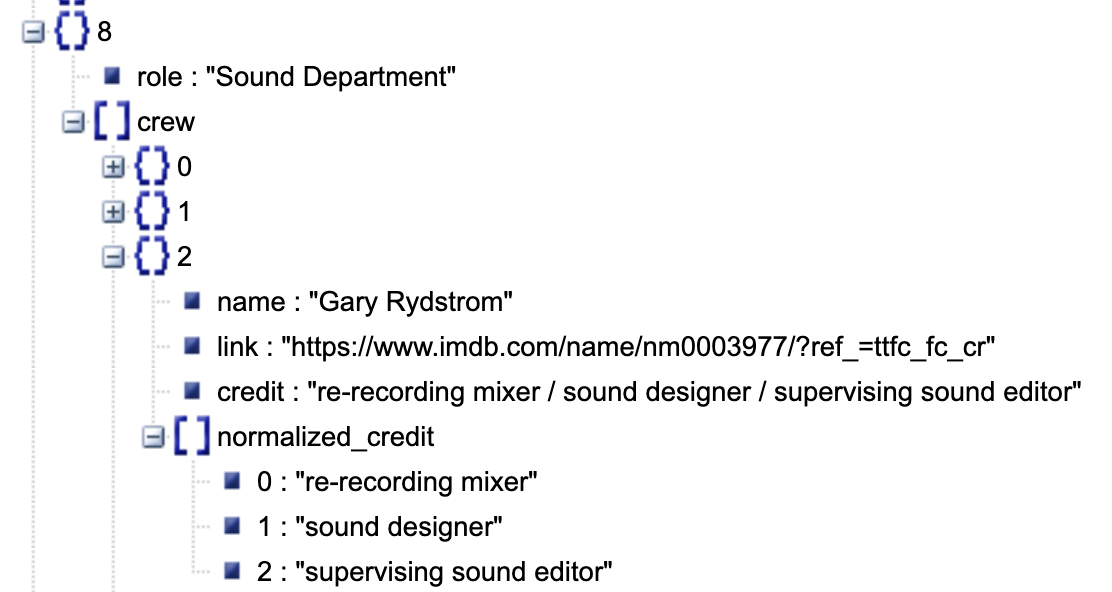
\includegraphics[width=0.5\linewidth]{soundRoles.png}
    \caption{Example of a crew member with multiple sub-roles.}
    \label{fig:soundRoles}
\end{figure}
\par
It is important to note that this process of normalization and filtering is not perfect, in large part due to the inconsistencies in IMDb data. In future research, it would be interesting to investigate how this data is recorded, who records it, and what guidelines are in place to manage the quality and accuracy of the data that is available.
\subsection*{Data Download}
Using the CSV file provided that contained the information for the 101 directors of interest, I was able to loop through each IMDb uri and extract the desired data, filtering and normalizing when necessary. It is important to note that, if the director had a lot of associated data, the download would timeout, so I integrated a method of rerunning the download for those problem IDs. This allowed me to download all 101 directors, only running the code once. 
\par
The result was a nested dictionary for each director that contained general information about the director, including their ID, race, gender, and whether they were within the top 20 highest-grossing directors in the dataset. Each director dictionary contained a key "complete\_credits". The associated value was another dictionary containing each of the movies the director directed and a nested dictionary containing information about the individual crew members who worked on each movie (see Figure \ref{directorSubset}). In addition to the crew information, each movie dictionary contained an "imdb\_details" key that contained additional details about the movie, including a description, the content rating, and a summary of the movie reviews. 

\begin{figure}
    \centering
    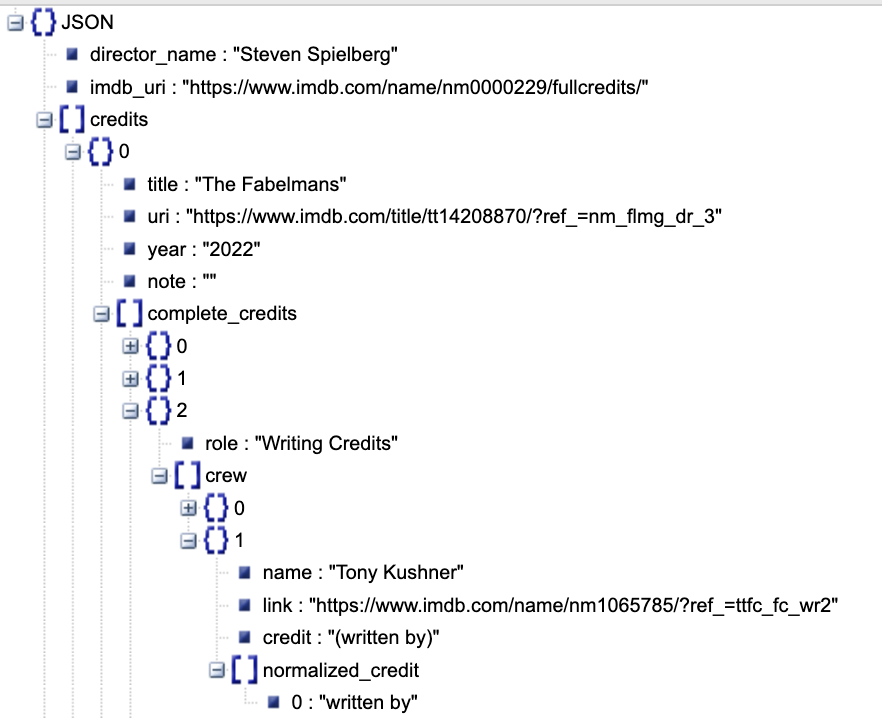
\includegraphics[width=0.5\linewidth]{directorSubset.png}
    \caption{Extract from Steven Spielberg's JSON file. This image captures the data for one crew member, Tony Kushner, for one of the films Spielberg directed, "The Fabelmans".}
    \label{fig:directorSubset}
\end{figure}

\section*{Network Generation}
\subsection*{Network Structure}
Our network model is made up of two distinct node types,\textbf{ director nodes (D)} and \textbf{crew nodes (C)}, each possessing different attributes, and two distinct edge types, director-director edges (D-D) and director-crew edges (D-C). The network itself is an undirected, weighted graph.

\subsection*{Nodes}
\textbf{Director nodes} possess the following attributes (see Figure 1 in the Appendix for a detailed table of director node attributes):
\begin{itemize}[itemsep=-5pt]
    \item role
    \item sex
    \item race
    \item labels (if applicable)
    \item total\_films
    \item collabs
\end{itemize}
\begin{figure}[h!]
    \centering
    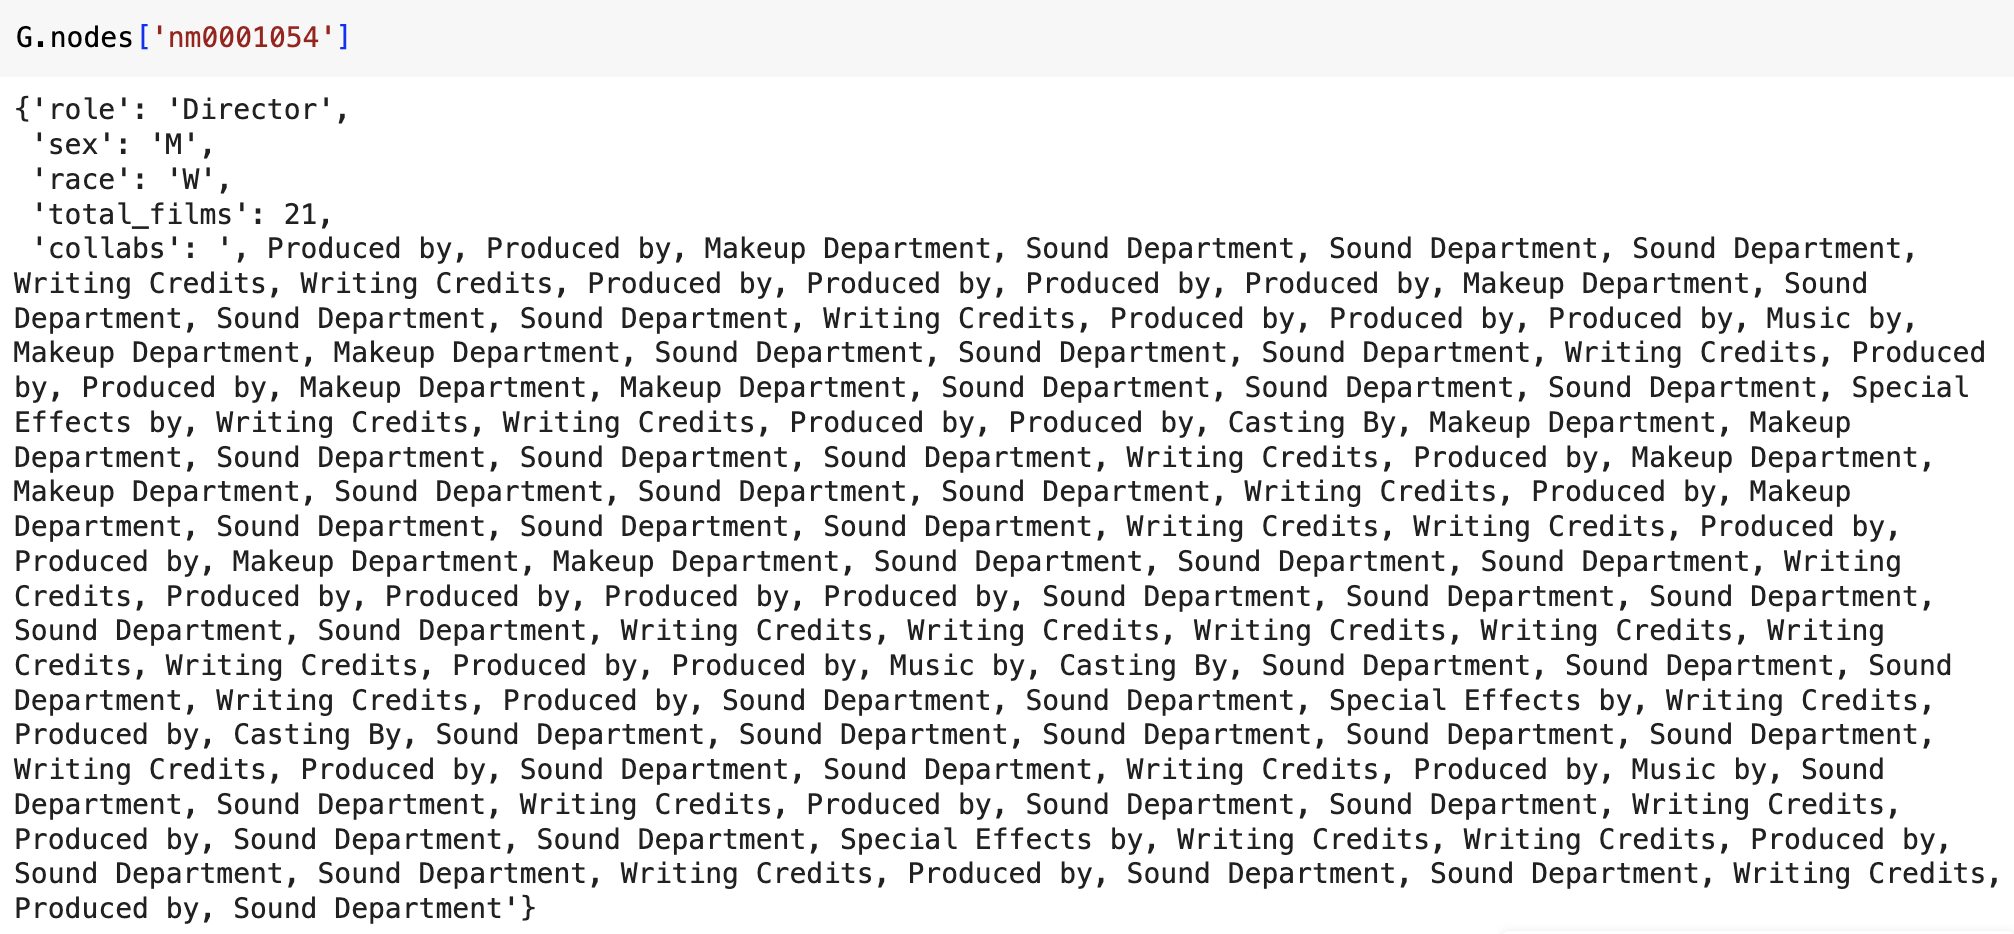
\includegraphics[width=0.5\linewidth]{director_node.png}
    \caption{An example output showing director node attributes.}
    \label{fig:dir_node}
\end{figure}

Whereas \textbf{crew member nodes }possess the following attributes (see Figure 2 in the Appendix for a detailed table of crew node attributes):
\begin{itemize}[itemsep=-5pt]
    \item roles
    \item subroles
    \item directors
    \item years
    \item total\_films
    \item total\_directors
    \item min\_year
    \item max\_year
    \item start\_role
    \item end\_role
    \item num\_roles
    \item num\_subroles
    \item role

\end{itemize}
\begin{figure}[h!]
    \centering
    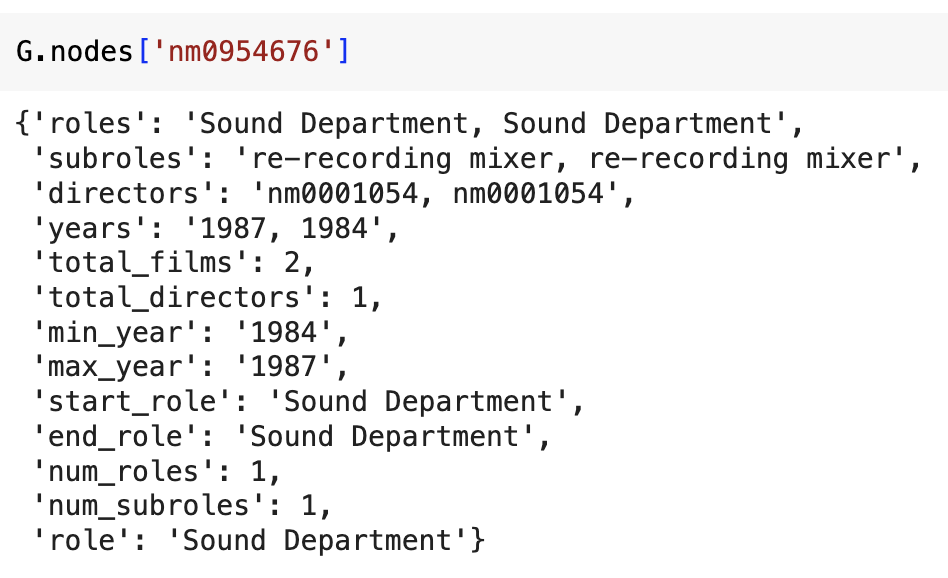
\includegraphics[width=0.5\linewidth]{crew_node.png}
    \caption{An example output showing crew node attributes.}
    \label{fig:crew-node}
\end{figure}

\subsection*{Links}
If a director and crew member worked together on a film, the two nodes are linked. Similarly, if a director worked under another director in a non-directing role, the two directors are linked. The only link type that does not exist in our network is crew-crew links. These could be discovered, however, were we to create a projection of the network linking together crew members if they worked with the same director.

\textbf{Director-Director links (D-D)}: Links between directors are weighted by the number of times the directors collaborated on films OTHER THAN co-directing (Ex: When Director A is a producer on a film Director B is directing, their edge weight increases by one. The edge is undirected, so it will also increase by one if Director B is a producer/writer/other non-director role on a film Director A is directing.) 
\begin{figure}[h!]
    \centering
    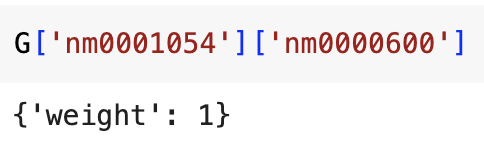
\includegraphics[width=0.25\linewidth]{DD_link.png}
    \caption{An example of a director-director link.}
    \label{fig:dd_link}
\end{figure}


\textbf{Director-Crew links (D-C)} possess two edge attributes: 'collaboration\_score' and 'weight'. 
\begin{enumerate}
    \item {Collaboration score }is the simpler of the two, defined as the percentage of the director's career (in \# of films) spent with a specific crew member. It is calculated by dividing the total number of collaborations between the director and the crew member (\# of times director's name is mentioned in the crew member node’s ‘directors’ attribute) by the total number of films directed by the director (‘total\_films” attribute in director node)

\begin{enumerate}
    \item \textit{collaboration\_score = (total collaborations \textbf{÷} total films) * 100\%}
    \item For a director who has directed 4 films and worked with a specific crew member 2 times, the link between the two nodes will have a collaboration\_score of 50\%.
\end{enumerate}
  
  \item The \textbf{weight} of the edge is similar to the collaboration score metric, but normalized to account for the significance of specific crew member roles. The calculation uses the same numerator as in the collaboration\_score metric (the total number of collaborations). However, rather than dividing by the total number of films directed by the director, we divide by the total number of times the director worked with someone in the same role as the crew member (including the crew member him or herself, however many times they worked with the director).  

We use this as the edge weight rather than the collaboration score or a raw count of total collaborations because certain crew roles are more time-consuming or rare than others. For example, there are usually considerably fewer writers on a film than there are members of the Sound Department, so the weights between directors and writers are generally greater than the weights between directors and sound crew. 
  \begin{enumerate}
      \item \textit{weight = (total collaborations \textbf{÷} role frequency) * 100\%}
      \item If the crew member's primary role is producer and they've worked with the director 2 times, the total\_collaborations value is 3. If the director has directed 3 films with 1 producer, 3 producers, and 4 producers respectively, the role frequency value is equal to 1 + 3 + 4 = 8. Therefore, the weight is equal to 2/8 = 1/4. 

  \end{enumerate}
    \end{enumerate}
\begin{figure}[h!]
    \centering
    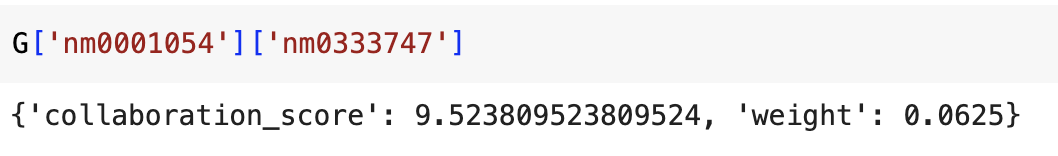
\includegraphics[width=0.5\linewidth]{DC_link.png}
    \caption{An example of a director-crew link.}
    \label{fig:dc_link}
\end{figure}


\subsection*{Assumptions and Justifications}
\begin{enumerate}
    \item The crew member's primary role is defined as the role they possessed most frequently over the course of their career. This is justified by the fact that the vast majority (97.4\%) of crew members remain in the same role for the entirety of their careers. 
    \item For one director-crew link, the edge weight calculation is invalid due to the fact that the director has not worked with anyone in the crew member's primary role and the crew member was working in a role other than their primary one while on the director's film. In this edge case, the edge weight is set equal to the collaboration score, which divides the number of collaborations by the total number of films. 
    \item Due to the overwhelming amount of niche subroles listed on IMDB, the usage of the more general role category is more effective for network generation. Relying on subroles to get adequate model results puts the model at a disadvantage because naming conventions of different roles differ across productions and many subrole titles are tailor-made for the movie itself. For example, crew members who wrote the book that a movie is based on are part of the Writing Credits role, but have subroles that include the specific book or movie title in them.
\end{enumerate}
        
\section*{Visualization}

\subsection*{Process Overview}
Below is an overview of the steps I followed to complete the visualization task. Within this task I contribute to the analysis section by writing a plan for how to address each research question and computing statistics in Gephi and NetworkX along the way. The visualizations are integrated into the analysis section for each research question.

\begin{enumerate}

\item Wrote a plan for how to answer each research question using specific network analysis techniques and a list of visualizations.
\item Identified the node and edge attributes required to achieve the visualizations to help with network generation.
\item Created a toy network with the required attributes to practice visualization in Gephi.
\item Planned additional visualizations like histograms, bar charts, and Sankey plots and described how each visualization helps to answer the research questions.
\item Wrote code to create plots using the toy network.
\item Applied code to finalized network generation and completed necessary troubleshooting.
\item Visualized networks in Gephi according to the written plan below, taking snapshots of the relevant filtered and unfiltered data.

\end{enumerate}

\subsection*{Chosen Visualization Methods}
A list of the visualizations chosen to answer each research question. After each question I provide reasoning for why I chose this visualization and the question it may answer. 

\textbf{Question 0: Characterize the director-crew network.}

\begin{itemize}
\item Number of movies per director? Histogram of the number of movies for the subset of director nodes.
\item Frequency of each role? Bar chart showing the count of each role across the entire network.
\item Number of crews? Histogram showing the number of unique crew members for each director.
\item Degree distribution? Histogram showing the degree distribution.
\end{itemize}

\textbf{Question 1: Measure how roles of crew members fluctuate.}

\begin{itemize}
\item Histogram showing the director influence distribution, calculated according to the described methods in the analysis section.
\item Career trajectory line plot case study: Pick a crew member and plot the number of movies they work on in each year to identify spikes after working with certain directors.
\end{itemize}

\textbf{Question 2: Measure how roles of crew members fluctuate.}

\begin{itemize}
\item Network visualization: A network with the node size = number of unique roles (num\_roles), node color = most frequent role (role), and edge size + edge color = constant. Take snapshots of the network filtered to different role types to answer the question: Which roles tend to work in other departments? Which crew member nodes have worked a uniquely large or small number of roles? 
\item Sankey diagram: Visualize the flow of role transitions from start of career (start\_role) to present (end\_role). How do roles change over the course of a career? Are there any roles that frequently lead to other roles (ex. Writer to producer)? 
\item Scatter plot of unique roles vs. total movies, colored by most frequent role: Do crew members tend to try new roles as they work on more movies, or maintain the same role?
\item Histogram of distribution of unique roles (num\_roles) for all crew members: This visualization will show trends in industry overall. How many unique roles do crew members have over their career?
\end{itemize}


\textbf{Question 3:  How widespread is the phenomenon of directors re-using the same crew? Do renowned directors (and women/minority directors) tend to work persistently with the same key collaborators compared to lesser recognized directors or a random Hollywood director?}

\begin{itemize}
\item Network visualizations: Node size = total number of films (to show how prolific the director is), node\_color: based on demographic attributes (sex, race, queer), edge size = normalized collaboration score (derived in the calculation mentioned above), and edge color = constant. Take snapshots of the network filtered to different demographics to answer the question: How do the ego networks of directors of different demographics compare in terms of their collaboration score?
\item Histograms of collaborations normalized by movies for each demographic: For each key demographic, make a histogram of the collaboration scores. How common is it for directors of each demographic to work with the same crew?
\item Scatter plot of number of movies vs. unique crew members, colored by demographics: This scatter plot will let us identify trends and possibly communities within demographics (clusters in the scatter plot). As directors make more movies, do they tend to use the same crew or many different crews?
\end{itemize}

The chosen networks visualizations leverage network analysis concepts like centrality, ego networks, and stylizing the network based on important node/edge attributes to quantify role fluctuation and collaboration patterns. Additional plots were selected to analyze career trajectories, role changes, and potential differences in director demographics. 


\section*{Analysis}
\subsection*{Overview of the Network}
There are 1415 featured movies in the network, 101 directors, and 4504 crew members. 

The directors in the network each have directed anywhere from 3 to 53 films, with an average of 14.009 movies per director.  

\begin{figure}[h!]
    \centering
    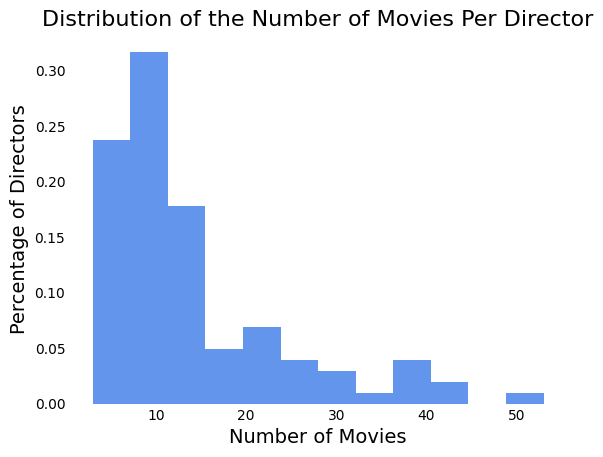
\includegraphics[width=0.33\linewidth]{0_histmoviesperdirector.png}
    \caption{A histogram showing the distribution of movies per director.}
    \label{fig:movies_hist}
\end{figure}

There are a total of 8 crew roles, with frequencies as shown in Figure 8.
\begin{figure}[h!]
    \centering
    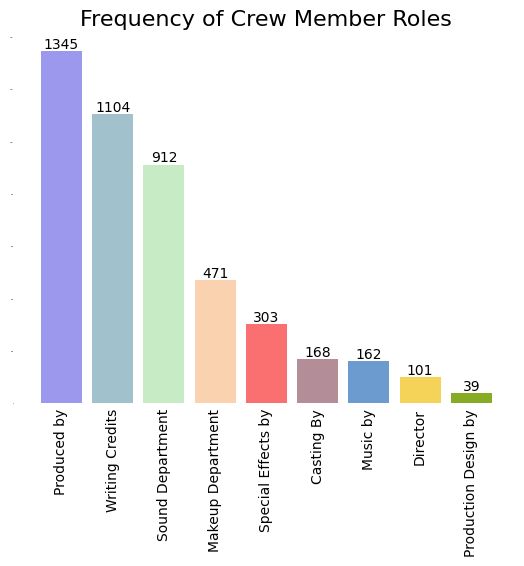
\includegraphics[width=0.33\linewidth]{0_crewmember_frequency.png}
    \caption{A bar chart showing the frequencies of crew roles.}
    \label{fig:bar-chart}
\end{figure}

The total number of unique crew members in a director's network is dependent on how many films they've directed, how large the crews were for said films, and the director's personal tendencies when it comes to rehiring the same crew members. All three of these aspects explain different proportions of the number of unique crew members depending on the director's specific circumstances. 
\begin{figure}[h!]
    \centering
    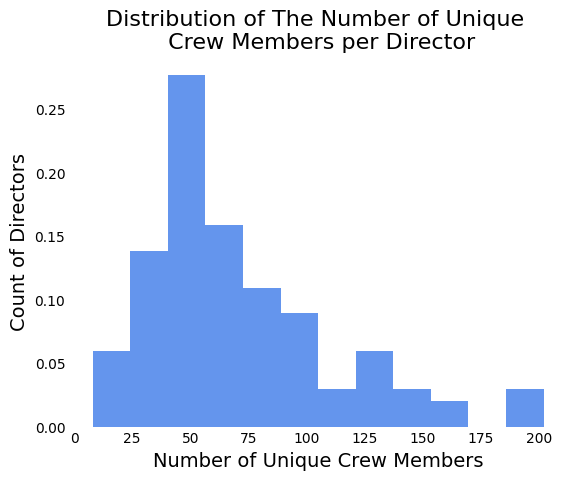
\includegraphics[width=0.33\linewidth]{0_histuniquecrewperdirector.png}
    \caption{A histogram showing the distribution of the number of unique crew members per director.}
    \label{fig:enter-label}
\end{figure}

\begin{figure}[!ht]
    \centering
    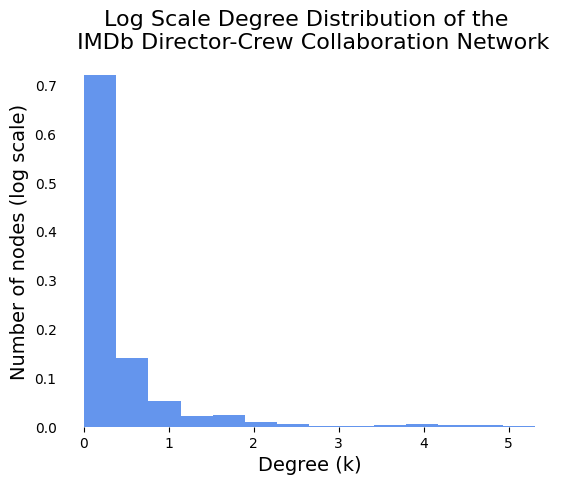
\includegraphics[width=0.33\linewidth]{0_degreedistlog.png}
    \caption{The degree distribution plot of the network (log scale).}
    \label{fig:log-label}
\end{figure}

The degree distribution of the network closely resembles what we would anticipate for a real-world network, with the plot following the power-law distribution. 

The network has an average shortest path length of 4.1956, an average clustering coefficient of 0.0159, and a density of 0.00067.




\subsection*{Question 1: Measure the influence of directors on crew members' careers.}

In order to measure the overall influence of directors on the future success of crew members, we calculate an influence metric. The methodology of the metric calculation is as follows:
\begin{enumerate}
    \item For each crew member, we aggregate the total number of movies they worked on per year. Data is placed in a dictionary with years as the keys and the total numbers of movies that the crew member worked on during each time period as the values.
    \item Iterating through each year chronologically, we track the change in total number of films. If the crew member sees a 50\% increase in the total number of films from one year to the next, we recognize the directors from the previous year as influential. (50\% increase indicates that the total number of films from the recent time period is 1.5 times the size of the total number of films from the previous time period).
    \item Directors' influence scores are then increased by a factor of (1/number of directors from previous year)*(number of movies in recent year/number of movies in previous year). 
    \begin{enumerate}
        \item Dividing by the number of directors that the crew member worked with in their time period leading up to the jump in their success allows for the credit to be equally distributed across directors. Given the cumulative nature of this metric (influence is an overall score that is increased any time crew members experience significant growth immediately after working with a director), using a normalized value is more effective than a raw count (ex: adding 1 to each director's influence score each time).
        \item Multiplying the 1/\# of directors portion by the ratio of recent time period movies to former time period movies allows for the influence metric to be scaled by the significance of career growth. For example, a director's influence score will be increased by a larger amount if their former crew member sees 500\% growth in the total \# of movies they work on in a year than if the crew member only sees a 50\% growth. 
    \end{enumerate}
\item Once all crew nodes have been accounted for, we create a table that contains director id numbers and their cumulative influence scores. 
\end{enumerate}
Here is a brief selection from the influence table calculated from our network:
\begin{table}[h!]
\centering
\begin{tabular}{|c|c|}
\hline
\textbf{Director} & \textbf{Influence} \\ \hline
nm0000142& 53.759852\\ \hline
nm0000229& 53.053355\\ \hline
nm0000165& 43.418332\\ \hline
...               & ...                \\ \hline
nm0001631& 0.550000\\ \hline
nm0036349& 0.390244\\ \hline
nm1883257& 0.202128\\ \hline
\end{tabular}
\end{table}

The directors have influence scores ranging from 0.2021 to 53.7599, with an average influence score of 11.435. This plot shows that the distribution of influence is skewed to the right, as many directors have influence scores of less than or equal to 15 and very few directors have influence scores higher than 15. 

\begin{figure}[ht]
    \centering
    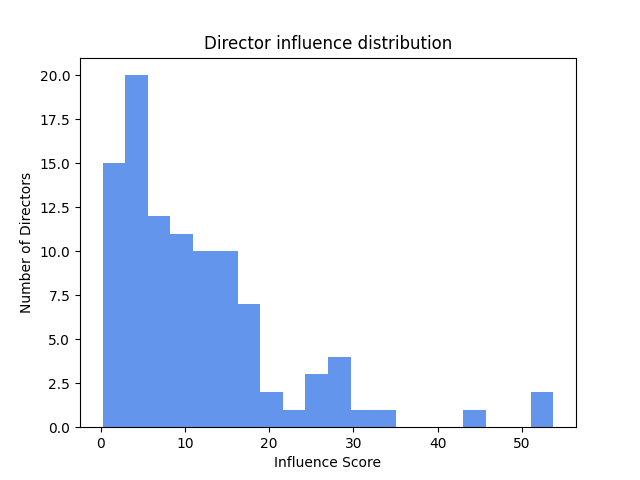
\includegraphics[width=0.33\linewidth]{1_influence_hist.png}
    \caption{A histogram showing the distribution of director influence values.}
    \label{fig:influence_hist}
\end{figure}

According to our calculations, the top ten most influential directors in order are:
\begin{enumerate}[itemsep=-6pt]
    \item Clint Eastwood (53.75985197273401)
    \item Steven Spielberg (53.05335525185566)
    \item Ron Howard (43.41833197931151)
    \item Ridley Scott (33.455846479716364)
    \item Tim Burton (31.72575494005538)
    \item Michael Bay (29.42764822060226)
    \item Robert Zemeckis (29.23757765500819)
    \item Martin Scorsese (28.077092366889264)
    \item Tyler Perry (27.29668109668107)
    \item Steven Soderberg (26.923324044376663)
\end{enumerate}

The directors with the lowest influence scores are Pablo Larrain, Andrea Arnold, Sarah Polley, Lynn Shelton, and Charles Burnett.  From a qualitative standpoint, these rankings make sense - specifically the most influential directors - as they are all quite well known and often work on films that require lots of crew, so they have very extensive networks and therefore a larger sample size of crew members who might display career growth after working with them. 

There are two primary drawbacks of this metric: the lack of normalization by crew member role type and dataset limitations.

Certain role types allow for crew members to be involved in more movies in the same time period than others. For example, makeup artists are able to work on more movies in a year than producers are, as producers are involved for the entire duration of the film-making process whereas makeup artists are only involved during the filming portion of the production. This is somewhat addressed by the usage of a threshold value rather than an exact number - we look for specific percentage increases, not point increases, which helps ensure credit is given to the crew members who are generally able to do to fewer films in a year. 

Because our dataset only contains well-known directors, it is likely that many crew members have credits from the years prior to their first time working with a director from our dataset as well as credits during the same time frame that are not accounted for in the network. The metric also fails if a crew member achieved significant career growth in the first three years and plateaued or didn't see that high of a rate of change again. 

However, we conclude that this metric is a valid way of evaluating the impact of directors on their crew members' career trajectories provided that we consider the values within the context of the limitations. 

\subsubsection*{Case study: Daniel Lepervanche (id = nm4951849)}

Daniel Lepervanche is a crew member whose primary role is working in the Sound Department. He experienced a substantial jump in his career between 2015 and 2016. 

\begin{figure}[h!]
    \centering
    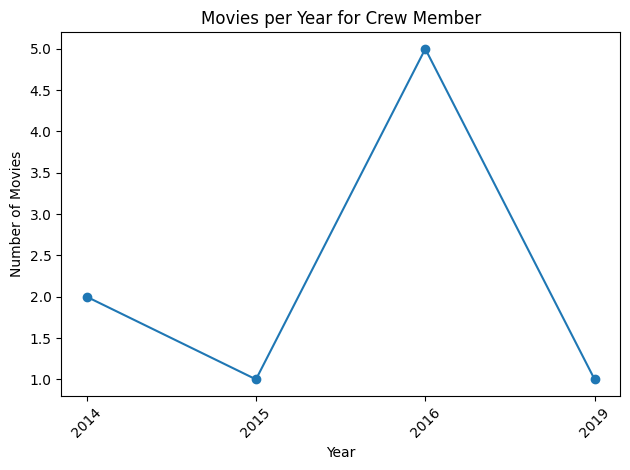
\includegraphics[width=0.5\linewidth]{1_career_traj.png}
    \caption{A line plot showing the career trajectory of a crew member, Daniel Lepervanche.}
    \label{fig:career_traj}
\end{figure}

In 2015, Lepervanche worked with Richard Linklater, who, according to our measure of influence, played some part in enabling Lepervanche to find significant success in the following year. Due to this instance, Linklater's influence score was increased by (5 films in 2016/1 film in 2015) * (1/1 director in 2015) = 5/1 * 1 = 5.

\subsection*{Question 2: Measure how the roles of crew members fluctuate.}

\noindent The whole group discussed the metric for crew member role fluctuation. Anna implemented the metrics and analyzed the visualizations.

\textbf{Results and Metrics}

We conclude that overall there is very little fluctuation in crew member roles, with the most common changes occurring in the writing and production departments. To answer this research question, we devised a metric to quantify how and how much a crew member's role changed. We derived the number of roles over dataset career as:

\begin{lstlisting}[language=Python,label=lst:copy]
attrs[name]['num_roles'] = len(np.unique(attrs[name]['roles'].split(', ')))

\end{lstlisting}
where ['roles'] is a list of all of the roles the crew member had on each movie for which their name id was listed. We were also interested to know which career changes were common, so we compared role fluctuations between departments using visualizations.

\textbf{Statistics and Visualizations Reveal That Crew Members Change Roles Infrequently}

The statistics and visualizations provide futher insights into how the roles of crew members fluctuate throughout their careers in the film industry. The two histograms (Figure 13, Figure 14) reveal that the vast majority of crew members had only one role (97.4\%) or one subrole (79.8\%). This trend indicates that there is very little role fluctuation among the crews of the 101 directors selected.

\begin{table}[H]
\centering
\begin{tabular}{|p{3cm}|p{5cm}|p{5cm}|}
\hline
 & Average number of unique roles & Average number of unique sub-roles \\ \hline
All crew members & 1.02 & 1.32 \\ \hline
Subset that experienced a role change & 2.02 & 2.48 \\ \hline
\end{tabular}
\end{table}

\begin{figure}[H]
    \centering
    % trim and clip are used to crop the image, trim=left bottom right top
    % width sets max width, height will be scaled appropriately
    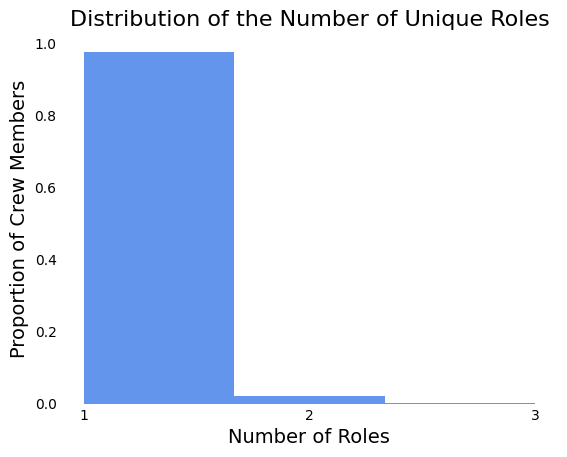
\includegraphics[clip,scale=0.7] {2_histnumroles.png}
    \caption{A histogram showing the distribution of number of unique roles.}
    \label{fig:sankey}
\end{figure}

\begin{figure}[H]
    \centering
    % trim and clip are used to crop the image, trim=left bottom right top
    % width sets max width, height will be scaled appropriately
    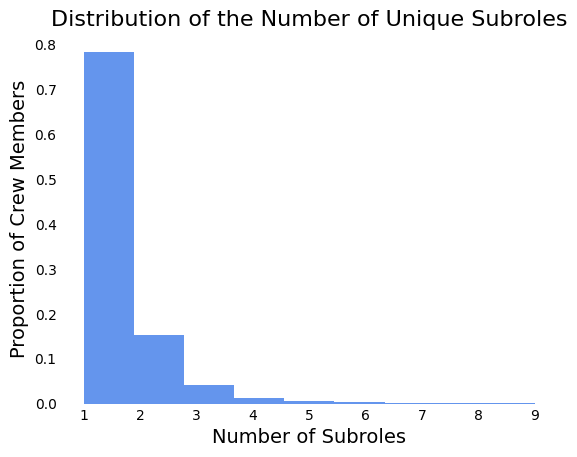
\includegraphics[clip,scale=0.7] {2_histnumsubroles.png}
    \caption{A histogram showing the distribution of number of unique subroles.}
    \label{fig:sankey}
\end{figure}


The Sankey plot affirms this conclusion by showing the changes between crew members' starting roles (the role on their first movie in the dataset) and their ending roles (the role on their most recent movie). 

\begin{figure}[H]
    \centering
    % trim and clip are used to crop the image, trim=left bottom right top
    % width sets max width, height will be scaled appropriately
    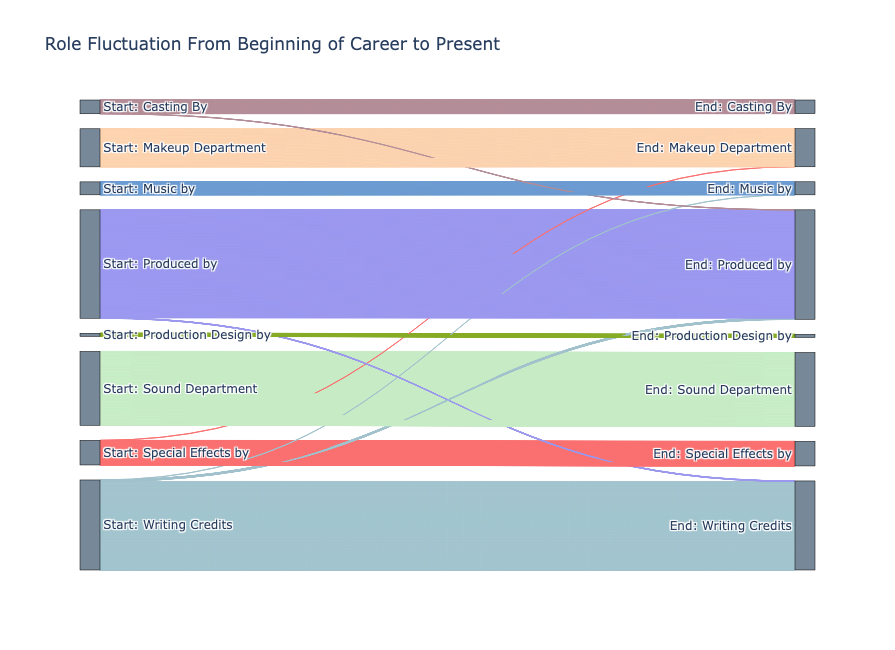
\includegraphics[clip,scale=0.5] {2_sankeyplot.png}
    \caption{A Sankey plot showing the flows between roles from the start of a crew member's career with the directors included to the present.}
    \label{fig:sankey}
\end{figure}


The plot (Figure 15) reveals that most crew members did not change roles from the start of their careers with the directors in the dataset to the present. The most common career change was from "Writing Credits" to "Produced by," though this is likely because these two roles are the most common overall. Notably, no one who started in the makeup, music, production design, or sound departments changed roles from the beginning of their career to the present. However, this diagram only captures the starting and ending roles, not any potential role changes in between.

\textbf{Roles Change More or Less Frequently Depending on the Department}

The network visualizations depict the director and crew member nodes according to their number of unique roles (node size) and their most frequent role (node color). One visualization shows a filtered version of all of the nodes with greater than five movies. A second version of the network is a collage of filtered networks of each role type (determined by the most common role the crew member has) to show the role fluctuations within certain roles.

\begin{figure}[H]
    \centering
    % trim and clip are used to crop the image, trim=left bottom right top
    % width sets max width, height will be scaled appropriately
    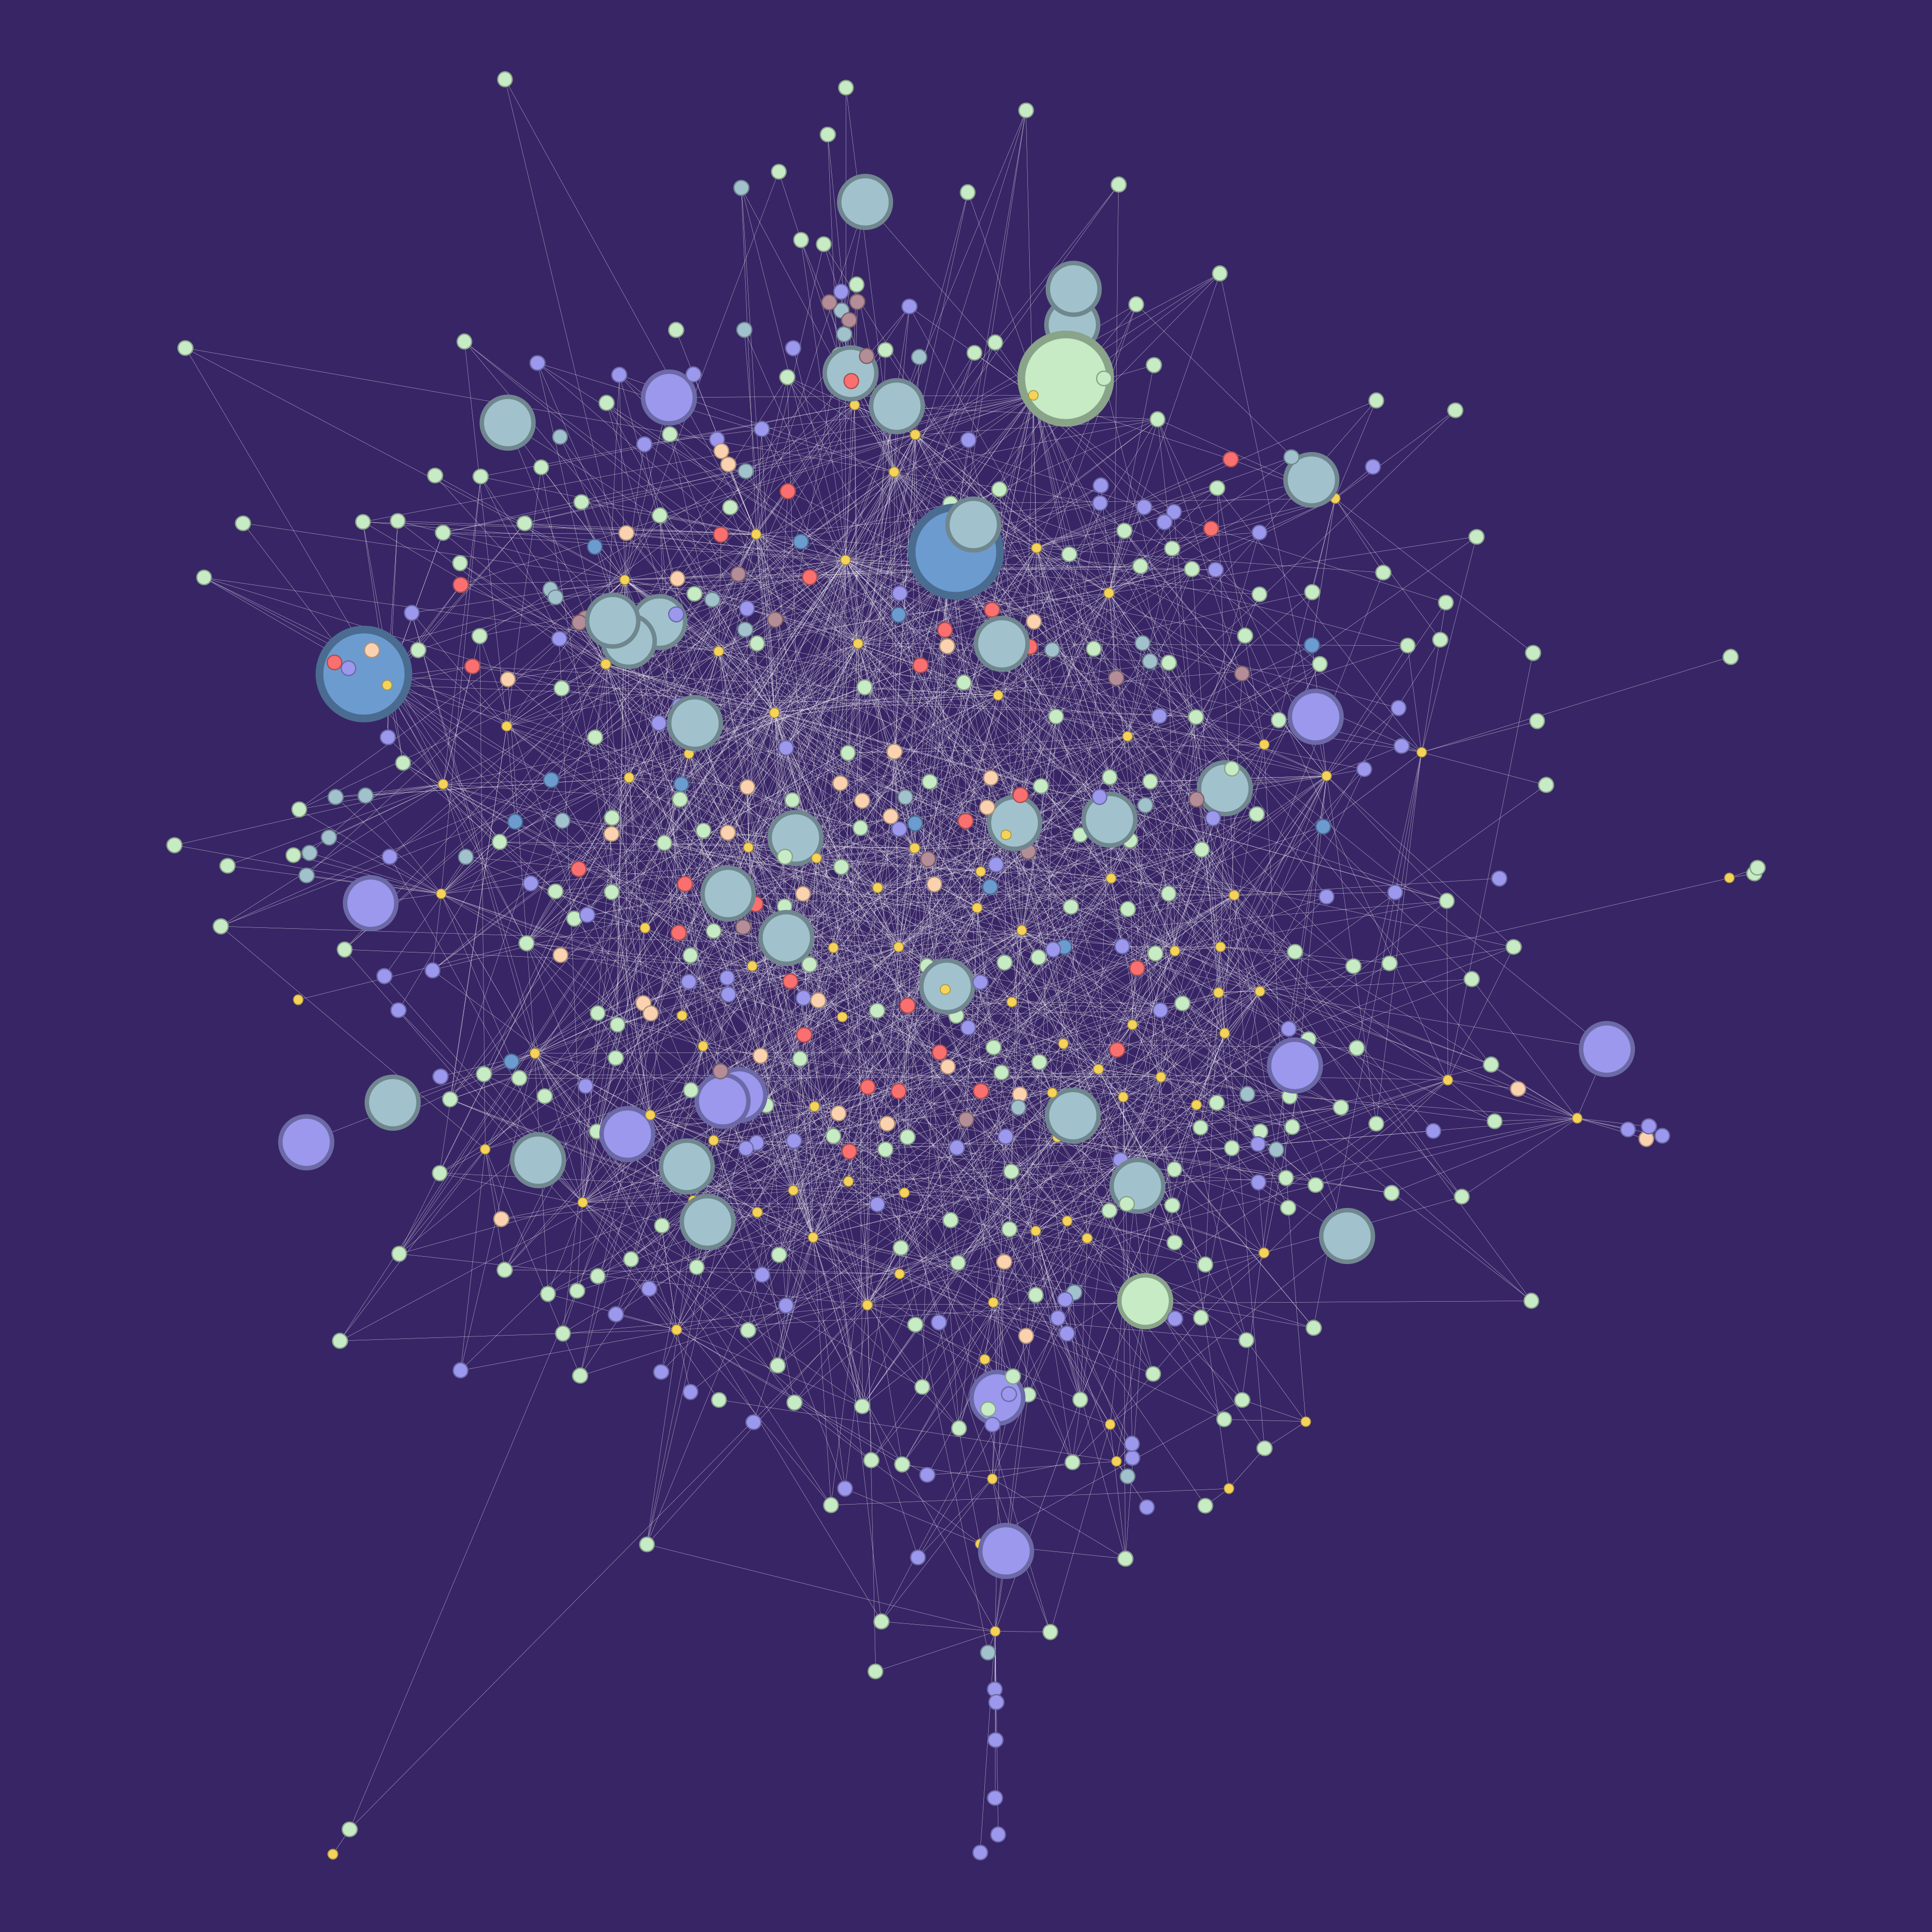
\includegraphics[clip,scale=0.12] {2_filterednetwork.png}
    \caption{IMDb network filtered to crew members who have worked on five or more movies, size based on number of roles}
    \label{fig:networkfiltered}
\end{figure}

\begin{figure}[H]
    \centering
    % trim and clip are used to crop the image, trim=left bottom right top
    % width sets max width, height will be scaled appropriately
    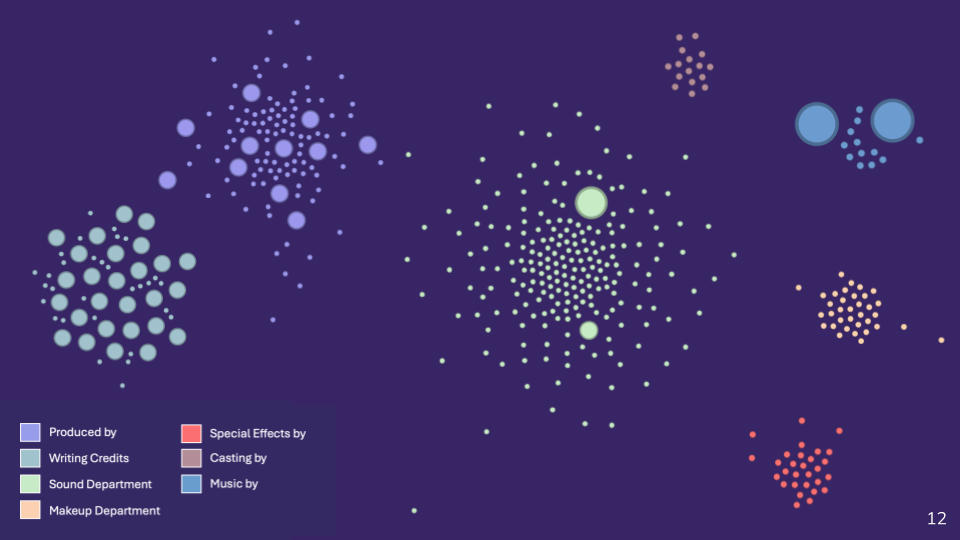
\includegraphics[clip,scale=0.5] {2_rolechangebyrole.png}
    \caption{A collage of number of unique roles by most frequent role type based on the filtered network.}
    \label{fig:networkorlechangebyrole}
\end{figure}

\begin{figure}[H]
    \centering
    % trim and clip are used to crop the image, trim=left bottom right top
    % width sets max width, height will be scaled appropriately
    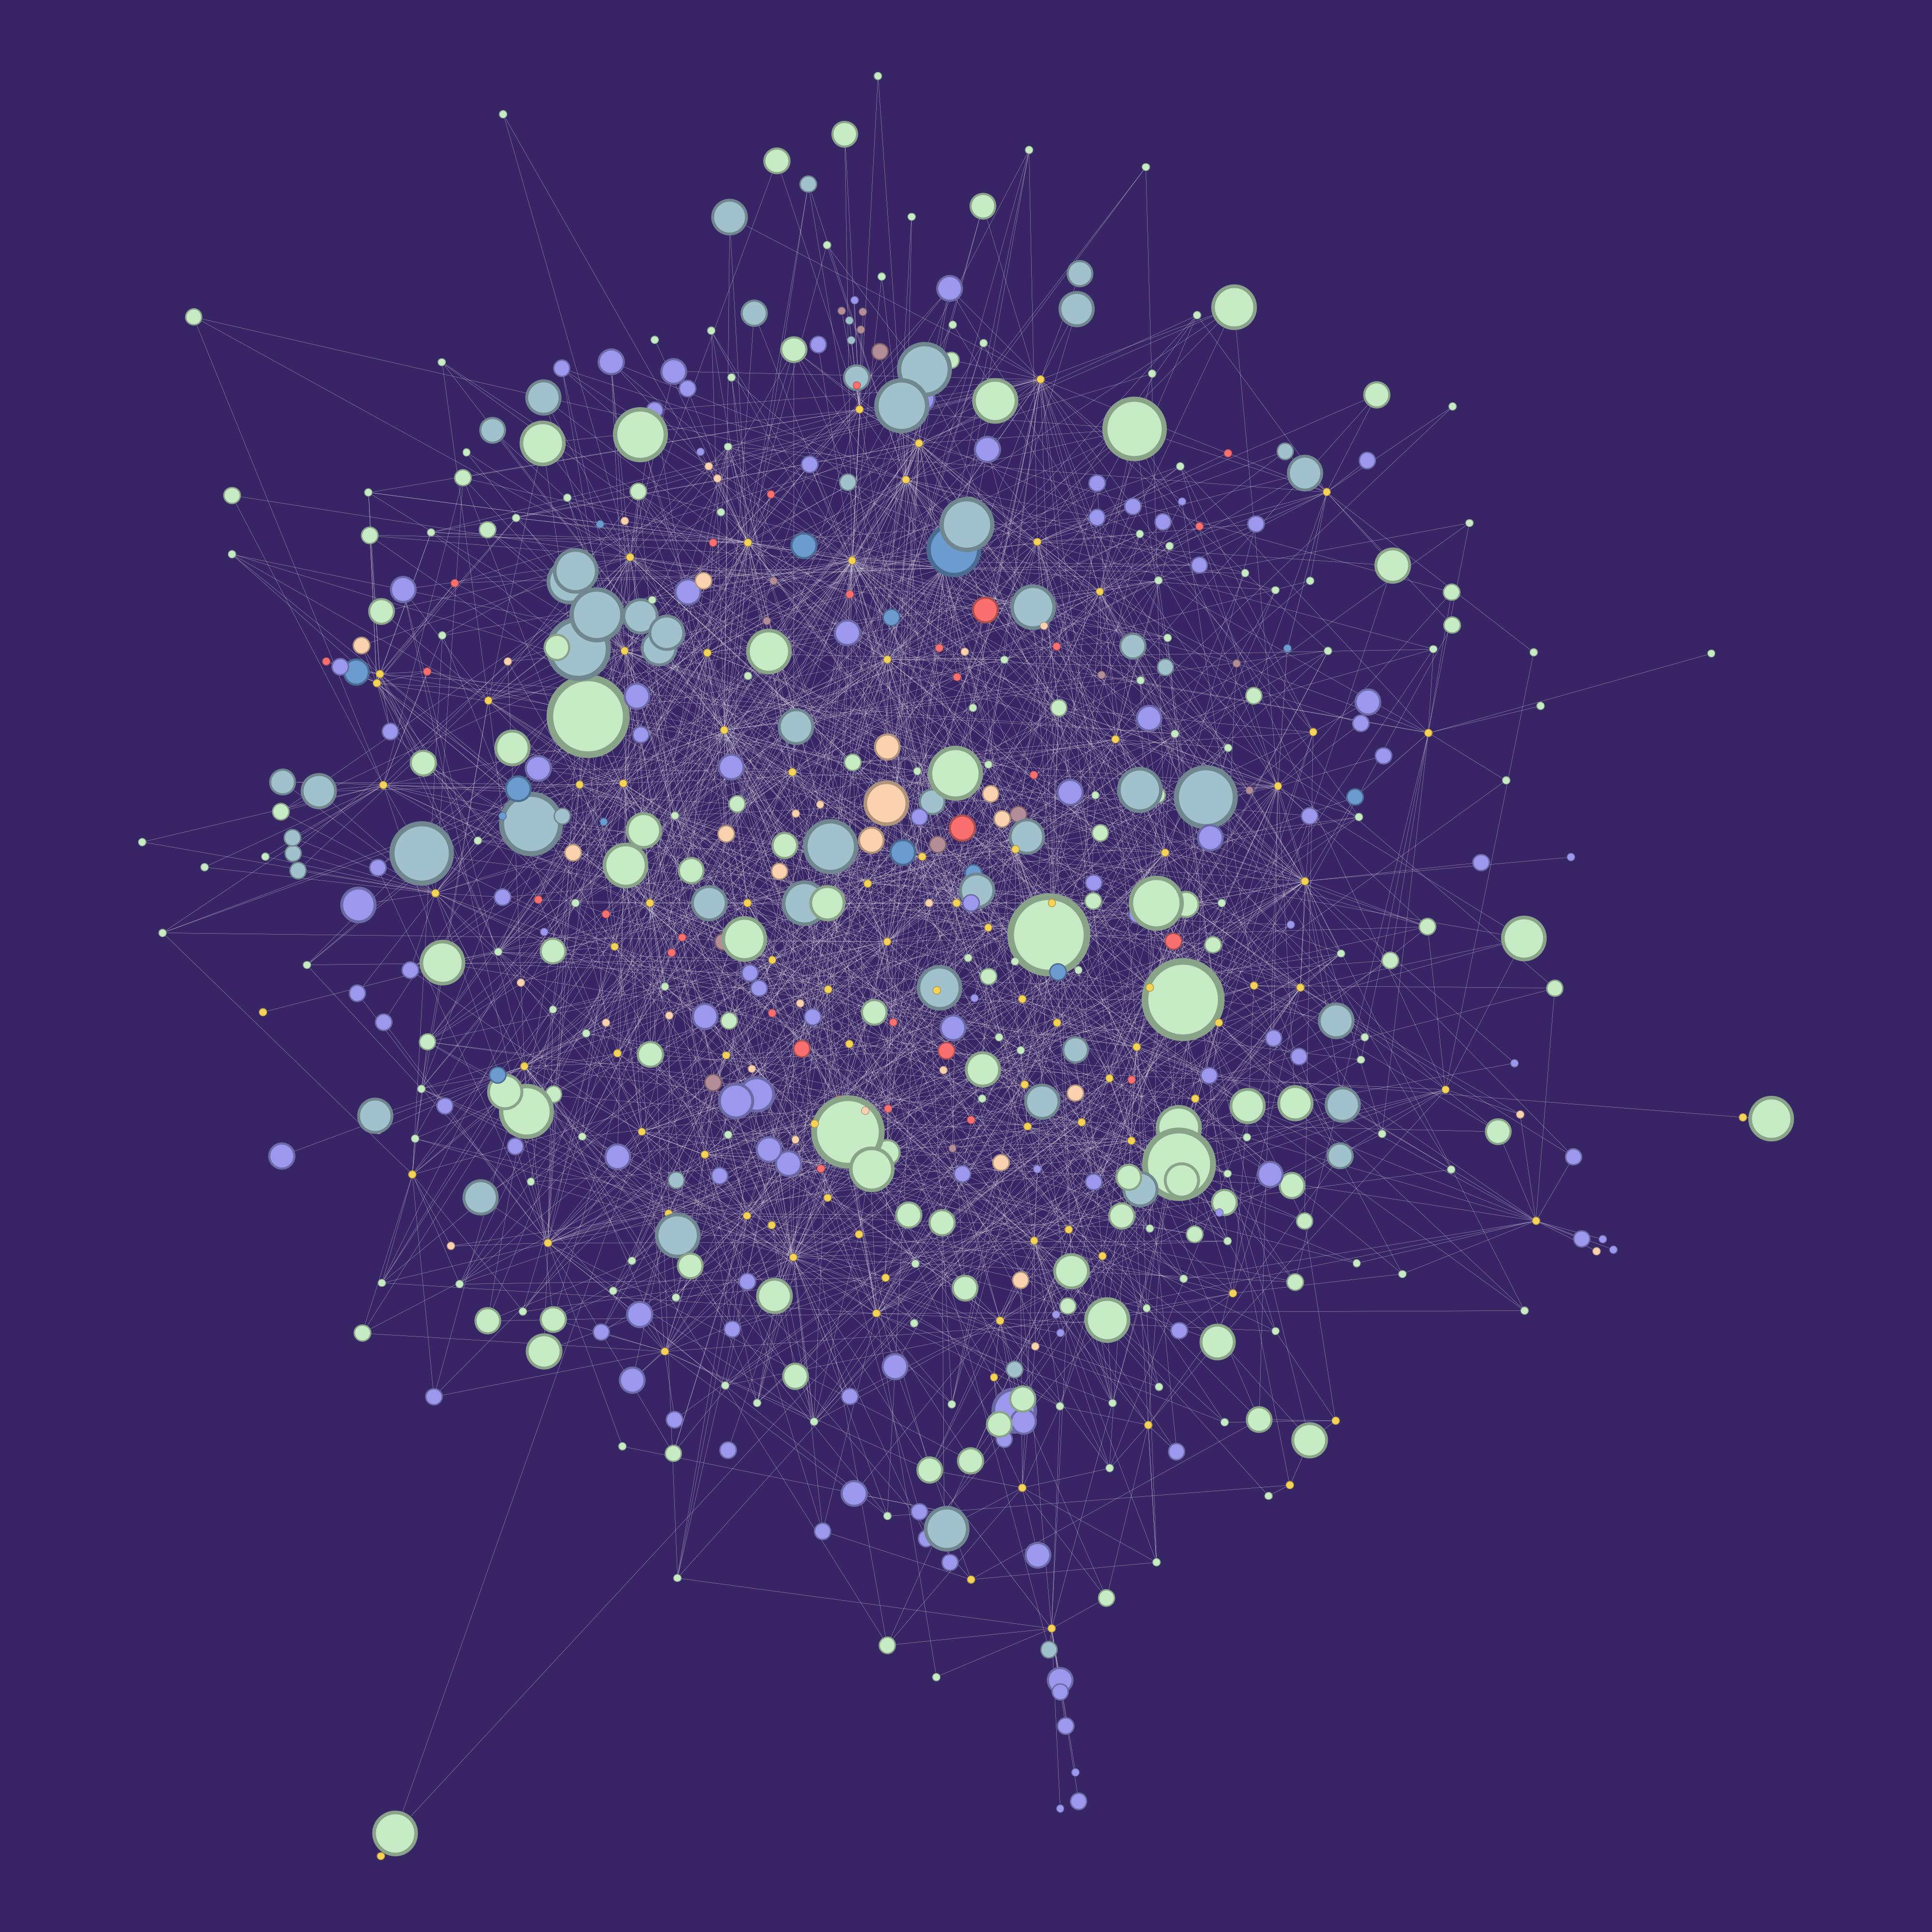
\includegraphics[clip,scale=0.12] {2_subroles_filtered.png}
    \caption{IMDb network filtered to crew members who have worked on five or more movies, size based on number of sub-roles}
    \label{fig:networkfiltered_roles}
\end{figure}


Filtering the network (Figure 16) to include only crew members who have worked on five or more movies allows us to analyze those who could have reasonably experienced a role change. Visually, we can see a trend where writers and producers were more likely to work in other departments throughout their careers, while those in makeup, casting, directing, special effects, production design, music, and sound rarely changed roles (see Figure 16, Figure 17). Production design crew members are excluded from Figure 17 because none worked in greater than five movies. One exception is the crew member with the most role changes, Hubert Bartholomae, who most frequently worked in the sound department but also music and special effects. 


A second version of the network (Figure 18) visualizes node size based on the number of unique subroles to show variation in roles both within and between departments. There is higher role fluctuation in the sound department and writing credits, some role fluctuation within producers and the makeup department, and little role fluctuation in all other departments. The network highlights crew members with particularly diverse roles over their careers and reveals trends in role fluctuations within departments.

\textbf{More Prolific Crew Members Tended to Have Fewer Role Changes}

Finally, the scatter plots (Figure 19, Figure 20) attempt to identify any trend between the number of movies a crew member works on and the number of unique roles they occupy. We theorized that as crew members work on more movies, they may 1. have the freedom to try new roles or 2. enter a role they are satisfied in and therefore stop trying new roles. 

\begin{figure}[H]
    \centering
    % trim and clip are used to crop the image, trim=left bottom right top
    % width sets max width, height will be scaled appropriately
    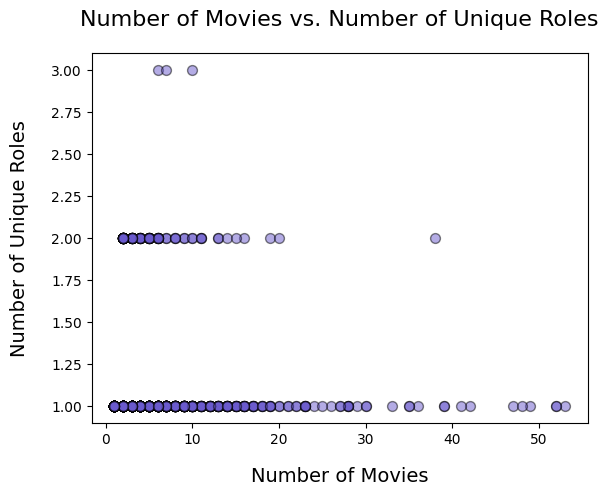
\includegraphics[clip,scale=0.8] {2_scattermoviesroles.png}
    \caption{A scatter plot showing the relationship between number of movies and number of unique subroles.}
    \label{fig:networkfilteredsubroles}
\end{figure}

\begin{figure}[H]
    \centering
    % trim and clip are used to crop the image, trim=left bottom right top
    % width sets max width, height will be scaled appropriately
    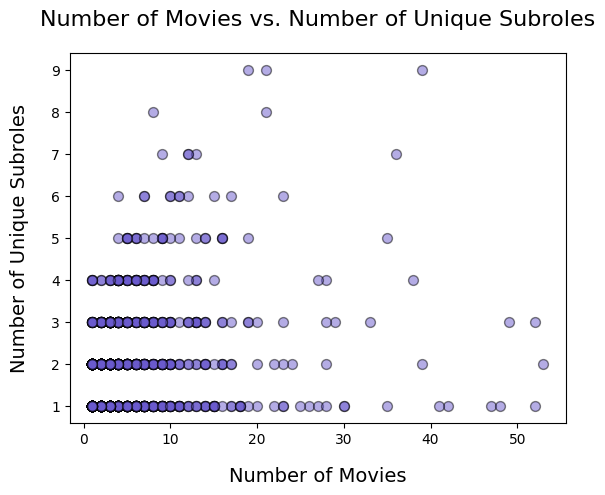
\includegraphics[clip,scale=0.8] {2_scattermoviessubroles.png}
    \caption{A scatter plot showing the relationship between number of movies and number of unique subroles.}
    \label{fig:networkfiltered}
\end{figure}

However, the random patterns in the data suggest no clear relationship. In fact, nodes representing crew members who have worked on the most movies often have fewer roles, indicating that finding and sticking to a niche role early in one's career may lead to more success or a more prolific career.

Overall, the visualizations consistently demonstrate that crew members in the film industry tend to specialize in a single role or department throughout their careers, with little role fluctuation over time. Exceptions to this trend are relatively rare, particularly among certain departments like sound and production design.


\subsection*{Question 3: How widespread is the phenomenon of directors re-using the same crew? Do renowned directors (and women/minority directors) tend to work persistently with the same key collaborators compared to lesser recognized directors or a random Hollywood director?}

\subsection*{Metrics for Directors Re-Using Crew}
To answer this research question, we devised a metric to quantify, for a single director, the likelihood of that director reusing a crew member.
\begin{enumerate}
\item We decided to use the "collaboration\_score" attribute from the network's Director-Crew links as the starting point for determining how often a director reuses the same crew. We chose this simpler attribute so that the collaboration score doesn't penalize a collaboration based on the number of people who held a specific role for a film. For example, we did not want the collaboration score for a specific sound designer to be diminished if the director worked on movies that required lots of sound designers. The specific calculation for this score is: 
\begin{equation} \label{eq:collaboration_score}
    CollaborationScore = \frac{TotalCollaborations}{Total Films Directed}\times100 
\end{equation}

\item Using this score, we were able to calculate the average collaboration score for each director in the network:
\begin{equation} \label{eq:avgCollaboration_score}
    Average Collaboration Score = \frac{\sum{CollaborationScores}}{Number of Collaborators}
\end{equation}

\item Once we obtained the average score for each director, we saved these scores in a dictionary format, with the director ID as the key and the average collaboration score as the value.
\end{enumerate}

\par
To determine whether different subgroupings of directors reused with crew members more than others, we first categorized the director IDs based on the general director details provided in the original CSV file using the following loop:

\begin{lstlisting}[language=Python, caption=Code used to categorize the director IDs based on characteristics including gender, race, and how renowned they are., label=lst:directorIDCategorization]
minorityDir = []
lesserKnownDir = []
renownedDir = []
womenDir = []
queerDir = []
maleDir = []
randomDir = []
for node, data in G.nodes(data=True):
    
    if data['role'] == 'Director':

        if 'labels' in data:
            renowned = data['labels']
            if renowned == 'H':
                renownedDir.append(node)
            elif renowned == 'Q':
                queerDir.append(node)
                lesserKnownDir.append(node)
        if 'sex' in data:
            sex = data['sex']
            if sex == 'F':
                womenDir.append(node)
            elif sex == 'M':
                maleDir.append(node)
        if 'race' in data:
            race = data['race']
            if race != 'W' and node not in minorityDir:
                minorityDir.append(node)
        if 'labels' not in data:
          lesserKnownDir.append(node)
\end{lstlisting}

Once the director IDs were classified, we were able to calculate the average collaboration score for the directors in each category. It is important to note that a potential limitation of this method is the varying number of directors in each category. In this dataset, there are 81 lesser-known directors, 20 renowned directors,   31 directors of color,  74 male directors, 27 female directors, and 7 queer directors. We also downloaded data for 100 random directors and calculated the average collaboration score for these directors.
\par
When calculating the scores, we encountered some irregularities among the random directors. Some of these directors, including Felix Girard (nm0320657), only directed one movie and some do not have any associated crew data. We decided to penalize the collaboration score for the directors who directed fewer movies since, if you only work on 1 movie, the current metric returns a collaboration score of 100\%. This does not accurately capture the idea of reusing the same crew. To account for this, we created a method of penalizing the collaboration scores for each director:
\begin{equation} \label{eq:avgCollaboration_score}
    PenalizedScore = ((Director Collab Score\times0.01) - \frac{1}{Total Films Directed^2 + 1})\times100
\end{equation}
By subtracting 1 over the squared number of films the director directed plus 1, we were able to decrease the collaboration score of directors who worked on fewer movies while not significantly affecting the scores of directors who worked on a large number of movies. For example, if a director only directed 2 films and had a collaboration score of 50\%, this penalty would change their score to 30\%. On the other hand, if a director who directed 50 films and had a collaboration score of 50\%, they would have a penalized collaboration score of 49.96\%. After these calculations, we calculated the average penalized collaboration score for each category of directors. The code below illustrates how this calculation was implemented in.

\begin{lstlisting}[language=Python, caption=Code used to penalize the collaboration score for each director in a category, then calculate the average collaboration score for that subset of directors., label=lst:calculatePenalizedScore] 
for k,v in dict_total_score.items():
    # account for directors who have a collaboration score of 0
    if v == 0:
      dir_AVERAGES[k] = 0
    else:
      # convert the collaboration score back to a decimal 
      # allows the penalization to have a larger effect
      v_decimal = v/100
      avgCollabBeforePen = v_decimal/id_count_dict[k]
      # due to inconsistencies in IMDb data, some directors had a collaboration score > 100%. 
      if avgCollabBeforePen > 1:
        avgCollabBeforePen = 1
        dir_AVERAGES[k] = ((avgCollabBeforePen)-(1/((total_films[k]**2)+1)))*100
      else:
        dir_AVERAGES[k] = ((avgCollabBeforePen)-(1/((total_films[k]**2)+1)))*100

  overall_average_collab = sum(list(dir_AVERAGES.values()))/len(list(dir_AVERAGES.values()))
\end{lstlisting}

\subsection*{Collaboration Score Results: Female and Minority Directors Have Higher Collaboration Scores than Other Categories}
Based on these calculations, which were finalized using the code in "crowley\_collaboration\_stats.py", we got the following results:

\begin{table}[h!]
\fontsize{11pt}{11pt}\selectfont
\centering
\begin{tabular}{| c | r | r | r |}
\hline
\thead{\textbf{Director Subset}} & \thead{\textbf{Min Collaboration Score}} & \thead{\textbf{Max Collaboration Score}} & \thead{\textbf{Average Collaboration Score}} \\
\hline
Female & 8.13 & 25.64 & 16.48 \\
\hline
Queer & 5.15 & 24.92 & 16.25 \\
\hline
Directors of Color & 3.94 & 30.41 & 14.26 \\
\hline
Lesser-Known & 3.79 & 30.41 & 13.16 \\
\hline
Random & 0 & 80.0 & 12.48\\
\hline
Renowned & 4.11 & 23.19 & 12.45 \\
\hline
Male & 3.79 & 30.41 & 11.76 \\
\hline
\end{tabular}
\caption{Summary of the collaboration scores for different categories of directors.}
\label{table:provinceClimateValues}
\end{table}

From this table, it is immediately clear that the phenomenon of directors reusing the same crew is not very widespread. The female directors in this dataset had the highest average collaboration score, 16.48. This means that, on average, female directors only worked with a specific crew member for 16.48\% of their movies. Female directors also had the highest minimum collaboration score, 8.13. This specific collaboration score was Mira Nair's (nm0619762) average collaboration score, so in this dataset, she was the female least likely to re-use the same crew. On the other hand, Sarah Polley (nm0001631) was the female most likely to reuse the same crew. On average, she works with a single crew member on 25\% of her films.
\par
Male directors had the lowest average collaboration score, 11.76. The second-lowest collaboration score was also for a male, Brian De Palma (nm0000361). The male director category did tie for the second-highest collaboration score, 30.41. The reason that this score ties with the highest average Lesser-Known director score and the highest average score for a director of color is that Ryan Coogler (nm3363032) falls into all three categories. This highlights a limitation of our method of calculating collaboration scores. However, it is interesting that there is such a stark difference between the collaboration patterns of women versus those of men.
\par
Another interesting pattern in these results is that two other categories of directors who can be classified under the "minority" director category, queer directors and directors of color, have the second and third-highest average collaboration scores, respectively. For queer directors, their average collaboration score is 16.25, only slightly lower than the average collaboration score for female directors. Their lowest collaboration score, 5.15, is also the second-highest minimum score. While the minimum score for directors of color is the third-lowest, the average score is the third-highest, 14.26. Based on the fact that the top-three average collaboration scores are associated with groups of minority directors, we infer that these directors maintain a tighter circle and prefer to work with people they've worked with previously when it is possible compared to other groups of directors.
\par
Another way we categorized the directors was based on whether they were renowned or not. Based on these calculations, renowned directors only had a slightly lower collaboration score, 12.45, compared to lesser-known directors 13.16. However, these scores have a limited ability to explain the phenomenon of reusing crew since the sample size of renowned directors is significantly smaller than that of lesser-known directors. 
\par
Comparing the scores of renowned directors to the average female director collaboration score, the average score for directors of color, and the average score for queer directors, the collaboration score of renowned directors is much lower. One reason for this is that renowned directors may have less control over the crew that they hire since the producers of high-budget films may exercise more control over the hiring process. Additionally, these renowned directors may attract a wider variety of people who want to work on their movies, therefore diversifying the crew they work with on each movie. Since women, people of color, and queer individuals are not as represented in the movie industry as directors, it also makes sense that these individuals may have built up a close circle of people who they work with. In future research, it would be interesting to calculate the clustering coefficient of subnetworks that include links between crew members to see whether crew members who work with underrepresented directors also work with one another more often. For the purposes of this project, we did not include links between crew members.
\par
Finally, we looked at the collaboration score for a network of random directors. This proved to be a bigger challenge than expected because many of these directors are not well-known or they do not have complete data in IMDb. Due to these limitations, the minimum and maximum collaboration scores are not very helpful for the analysis since they are so extreme, 0 and 80, respectively. However, the average collaboration score indicates that random directors are not as likely to reuse the same crew as the female directors, directors of color, queer directors, or lesser-known directors overall. Interestingly, based on this metric, the random directors had a slightly higher average collaboration score than renowned directors, but only by 0.03. Future tests using additional random directors would be beneficial to improve our confidence in these findings.
\par
To zoom in on the relationship between the director's race/ethnicity and the number of unique crew members they used in comparison to the total number of movies they made, we created a scatter plot. Based on this plot, it is clear that White directors direct more movies on average than directors of other races/ethnicities, but they also use a larger number of crew members. The majority of the directors of color use fewer unique crew members compared to white directors with a similar number of movies. The maximum number of crew members associated with a White director is 200, while the maximum number of crew members associated with a Black director is only about 135. Interestingly, Black directors who directed a higher number of movies (approximately 40) worked with a maximum of 125 crew members, while White directors working on a similar number of movies worked with up to 200 crew members. This could be due to White directors directing larger-scale movies, but it could also be due to Black directors re-using crew members. 
\par
Similar patterns exist for the other categories of directors, with Asian directors working with a maximum of about 110 crew members, Indigenous directors working with a maximum of approximately 75 crew members, and Latin American directors working with approximately 110 directors. All of these categories for directors of color illustrate that directors of color direct fewer movies than many White directors. In some cases, the low number of crew members is solely due to the smaller number of movies, but for directors who worked on similar numbers of movies, directors of color, particularly Black directors, work with fewer crew members.
\begin{figure}[H]
    \centering
    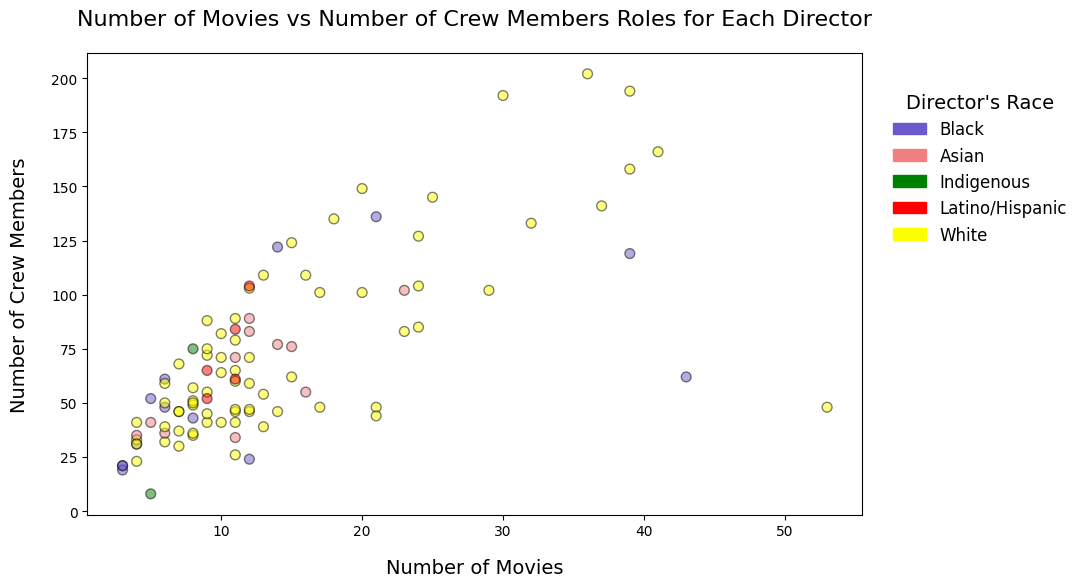
\includegraphics[width=350pt, scale=0.5] {3_scattermoviescrewrace.png}
    \caption{A scatter plot illustrating the relationship between the number of movies a director directed and the total number of crew members they used, based on director race/ethnicity.}
    \label{fig:raceScatter}
\end{figure}

Next, we compare the relationship between the director's gender and the number of unique crew members they used in comparison to the total number of movies they made. From the scatter plot in Figure \ref{fig:genderScatter}, it is immediately apparent that male directors direct more movies than female directors. However, when comparing male and female directors who directed the same number of movies, especially around 11 movies, the female directors worked with slightly fewer crew members. This slight difference highlights the fact that the reuse of crew is not incredibly common, but it is more common among female directors than male directors.

\begin{figure}[H]
    \centering
    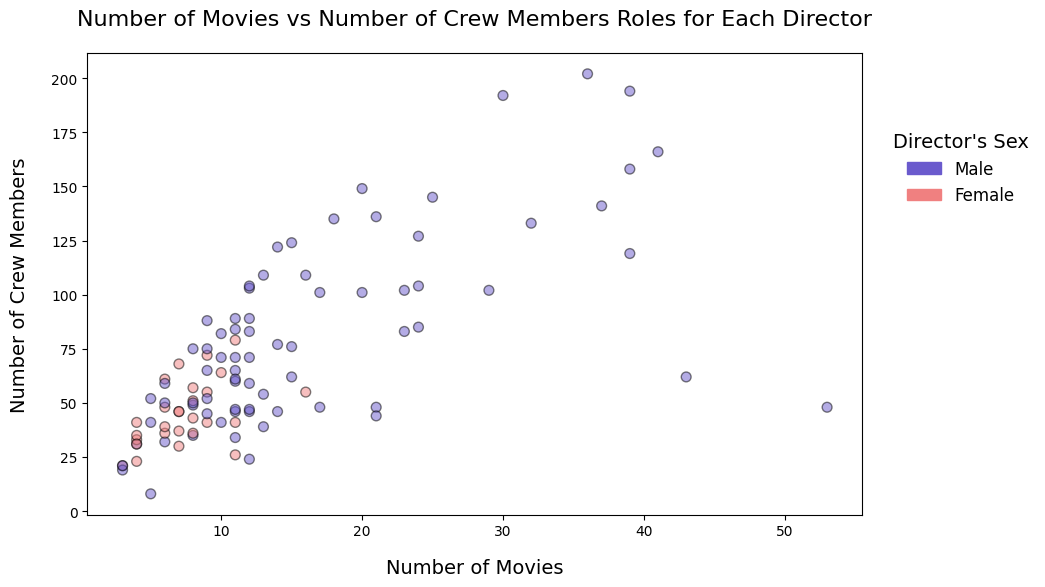
\includegraphics[width=350pt, scale=0.5] {3_scattermoviescrewgender.png}
    \caption{A scatter plot illustrating the relationship between the number of movies a director directed and the total number of crew members they used, based on director gender.}
    \label{fig:genderScatter}
\end{figure}
Based on all of these observations, we wanted to visualize these networks to see how directors related to their crew members. Figure \ref{fig:asianEgo} illustrates the network of Asian directors and their crew members. This network has a small number of directors, which allows us to see that there are clear hubs where specific directors are working with a relatively small number of crew members. Similarly, Figure \ref{fig:blackEgo} shows the network of Black directors. Once again, this network is relatively sparse and the director nodes have distinct communities, implying that the director reuses the crew for their movies. Figure \ref{fig:indigenousEgo} illustrates the network of Indigenous directors, which is very small. These two directors work with a small number of crew members, so it is likely that, if they have directed multiple movies, they are reusing crew. Figure \ref{fig:latinAmericanEgo} illustrates a similar pattern to the previous three networks and has about 3-4 distinct communities of crew members.
\begin{figure}[H]
    \centering
    \includegraphics[width=250pt,,scale=0.5] {3_asian_egonetwork.jpg}
    \caption{A network illustrating the relationships between Asian directors and their crews.}
    \label{fig:asianEgo}
\end{figure}
\begin{figure}[H]
    \centering
    \includegraphics[width=250pt, scale=0.5] {3_black_egonetwork.jpg}
    \caption{A network illustrating the relationships between Black directors and their crews.}
    \label{fig:blackEgo}
\end{figure}
\begin{figure}[H]
    \centering
    \includegraphics[width=250pt, scale=0.5] {3_indigenous_egonetwork.jpg}
    \caption{A network illustrating the relationships between Indigenous directors and their crews.}
    \label{fig:indigenousEgo}
\end{figure}
\begin{figure}[H]
    \centering
    \includegraphics[width=250pt, scale=0.5] {3_latinamerican_egonetwork.jpg}
    \caption{A network illustrating the relationships between Latin American directors and their crews.}
    \label{fig:latinAmericanEgo}
\end{figure}

\par
In comparison, the network of White directors (see Figure \ref{fig:whiteEgo}) does not have the same easily distinguishable communities. This is mainly due to the fact that the network is so large that it is difficult to see any of granular details. The edge weights are also much thinner, indicating fewer collaborations (taking the role frequency into account). In the previous networks, many of the edges were very thick, indicating a higher frequency of a crew member working with a director (based on their specific role).
\begin{figure}[H]
    \centering
    \includegraphics[width=250pt, scale=0.5] {3_white_egonetwork.jpg}
    \caption{A network illustrating the relationships between White directors and their crews.}
    \label{fig:whiteEgo}
\end{figure}


We can see a similar pattern when comparing the female and male networks. In Figure \ref{fig:femaleEgo}, the female director network, there are more discernable communities within the network than there are in Figure \ref{fig:maleEgo}, the network of male directors. However, it is somewhat difficult to solely compare the visualizations because the network of male directors has significantly more nodes than the network of female directors.
\begin{figure}[H]
    \centering
    \includegraphics[width=250pt, scale=0.5] {3_female_egonetwork.jpg}
    \caption{A network illustrating the relationships between female directors and their crews.}
    \label{fig:femaleEgo}
\end{figure}
\begin{figure}[H]
    \centering
    \includegraphics[width=250pt, scale=0.5] {3_male_egonetwork.jpg}
    \caption{A network illustrating the relationships between male directors and their crews.}
    \label{fig:maleEgo}
\end{figure}

Lastly, it is interesting to analyze the high-grossing director network (see Figure \ref{fig:highEgo}). This network has relatively discernible communities, but also has many crew nodes that are connected to more than one director and the director communities are relatively large. This network has similarities to both the male and female networks, almost falling in a middle ground between the two, which is interesting since the collaboration score of high-grossing directors is between that of male and female directors, although it is closer to that of male directors.
\begin{figure}[H]
    \centering
    \includegraphics[width=250pt, scale=0.5] {3_highgrossing_egonetwork.jpg}
    \caption{A network illustrating the relationships between high-grossing directors and their crews.}
    \label{fig:highEgo}
\end{figure}
\section*{Reflection}
Overall, analyzing networks of directors and their crew members reveals a significant amount of data about the movie industry and social patterns as a whole. Within this dataset, there are clear patterns of prevalence of directors based on gender and race, with White males being the most common type of director. Acknowledging this, it is important to consider how the identity of a director impacts the stories they are telling through their movies. Whose voices are heard? Whose stories still need to be told?
\par
Future iterations of this research should consider additional characteristics of the crew members, including gender and race, to determine whether the patterns found for directors hold for other roles. This analysis would also allow researchers to determine whether directors tend to work with crew members similar to them.

In our quantification of director influence, we discovered that directors with larger, more extensive networks had greater influence scores because they had interacted with more crew members and therefore had a larger sample of people to potentially experience a jump in success after working with them. This fails to take into account the consistency of a director's work with a crew member, as success can be additionally categorized by the consistency a crew member experiences in their careers.  This would be a potential area for future research and improving the robustness of the current influence metric.

Network and data visualizations also revealed that the majority of crew members work within the same role for all movies with the directors in the dataset. Could this be because the directors are more well known and thus hire people who are already well established, or is phenomenon also true of early-career crew members? 
Future research could investigate crew member role fluctuations for less well known directors or include variables to quantify career stage. Another future research direction could explore how role fluctuation changes within certain departments. Why do certain departments see more mobility than others? How do sub-roles vary within departments? 




\section*{References}

\begin{itemize}
    \item {NetworkX, \url{https://networkx.org/documentation/stable/reference/generated/networkx.classes.function.get_node_attributes.html}}
    \item {NetworkX, \url{https://networkx.org/documentation/stable/reference/generated/networkx.classes.function.number_of_edges.html}}
    \item {How to pass a list as a command-line argument with argparse?, \url{https://www.geeksforgeeks.org/how-to-pass-a-list-as-a-command-line-argument-with-argparse/}}
    \item {How do I print the key-value pairs of a dictionary in python, \url{https://stackoverflow.com/questions/26660654/how-do-i-print-the-key-value-pairs-of-a-dictionary-in-python}}
    \item {Find the keys using the values with some conditions in a dictionary using python?, \url{https://stackoverflow.com/questions/57412372/find-the-keys-using-the-values-with-some-conditions-in-a-dictionary-using-python}}
    \item {Select network nodes with a given attribute value, \url{https://stackoverflow.com/questions/31922917/select-network-nodes-with-a-given-attribute-value}}
    \item {How can I create a NetworkX subgraph from nodes with specific degree?, \url{https://stackoverflow.com/questions/54993898/how-can-i-create-a-networkx-subgraph-from-nodes-with-specific-degree}}
    \item {NetworkX, \url{https://networkx.org/documentation/stable/reference/classes/generated/networkx.Graph.subgraph.html}}
    \item {Why does argparse give me a list-in-a-list?, \url{https://stackoverflow.com/questions/5176846/why-does-argparse-give-me-a-list-in-a-list}}
    \item {How to pass and parse a list of strings from command line with argparse.ArgumentParser in Python?, \url{https://stackoverflow.com/questions/43786174/how-to-pass-and-parse-a-list-of-strings-from-command-line-with-argparse-argument}}
    \item {NetworkX Documentation get\_node\_attributes, \url{https://networkx.org/documentation/stable/reference/generated/networkx.classes.function.get_node_attributes.html}}
    \item {NetworkX Documentation Degree Analysis, \url{https://networkx.org/documentation/stable/auto_examples/drawing/plot_degree.html}}
    \item {What is a good measure of strength of a link and influence of a node?, \url{https://stackoverflow.com/questions/2815218/what-is-a-good-measure-of-strength-of-a-link-and-influence-of-a-node}}
    \item {Measure of influences in social networks
    , \url{https://www.sciencedirect.com/science/article/abs/pii/S1568494620307961}}
    \item {Convert series returned by pandas.Series.value\_counts to a dictionary, \url{https://stackoverflow.com/questions/29403192/convert-series-returned-by-pandas-series-value-counts-to-a-dictionary}}
    \item {Network X Documentation read\_gexf, \url{https://networkx.org/documentation/stable/reference/readwrite/generated/networkx.readwrite.gexf.read_gexf.html}}
    \item {Select nodes and edges form networkx graph with attributes, \url{https://stackoverflow.com/questions/45350222/select-nodes-and-edges-form-networkx-graph-with-attributes}}
    \item {How can I make a blank subplot in matplotlib?, \url{https://stackoverflow.com/questions/10035446/how-can-i-make-a-blank-subplot-in-matplotlib}}
    \item {GitHub: Resizing edge sizes changes edge weight values, \url{https://github.com/gephi/gephi/issues/180}}
    \item {Normed histogram y-axis larger than 1, \url{https://stackoverflow.com/questions/61881175/normed-histogram-y-axis-larger-than-1}}
    \item {argparse — Parser for command-line options, arguments and sub-commands, \url{https://docs.python.org/3/library/argparse.html}}
    \item {Appending into a List in Python Dictionary, \url{https://www.geeksforgeeks.org/appending-to-list-in-python-dictionary/}}
    \item {How do I create a dictionary with keys from a list and values defaulting to (say) zero?, \url{https://stackoverflow.com/questions/3869487/how-do-i-create-a-dictionary-with-keys-from-a-list-and-values-defaulting-to-say}}
    \item {Get all edges linked to a given node in a networkx graph, \url{https://stackoverflow.com/questions/33078907/get-all-edges-linked-to-a-given-node-in-a-networkx-graph}}
    \item {Iterating over dictionaries using 'for' loops, \url{https://stackoverflow.com/questions/3294889/iterating-over-dictionaries-using-for-loops}}
    \item {python list comprehension with multiple 'if's, \url{https://stackoverflow.com/questions/15248272/python-list-comprehension-with-multiple-ifs}}
    \item {How to check if a key exists in a Python dictionary, \url{https://www.educative.io/answers/how-to-check-if-a-key-exists-in-a-python-dictionary}}
    \item {Python: count repeated elements in the list, \url{https://stackoverflow.com/questions/23240969/python-count-repeated-elements-in-the-list}}
    \item {Parsing boolean values with argparse, \url{https://stackoverflow.com/questions/15008758/parsing-boolean-values-with-argparse}}

\end{itemize}


\section*{Appendices}
\begin{table}
\textbf{Figure 1 - Director node attributes}
\centering
\begin{tabular}{|>{\raggedright\arraybackslash}p{0.2\linewidth}|>{\raggedright\arraybackslash}p{0.2\linewidth}|>{\raggedright\arraybackslash}p{0.35\linewidth}|>{\raggedright\arraybackslash}p{0.25\linewidth}|}
\hline
\textbf{Attribute name}& \textbf{Object type}& \textbf{Definition}& \textbf{Sample attribute value}\\
\hline
role & string & The primary role of the node, ‘director’ for all director nodes & ‘director’ \\
\hline
sex & string & Sex of the director & ‘F’ for female, ‘M’ for male \\
\hline
race & string & Racial identity of the director & ‘B’ for Black, ‘L’ for Latino, ‘A’ for Asian, ‘I’ for Indigenous, ‘W’ for white \\
\hline
labels (if applicable) & string & ‘H’ if the director is one of the top 20 highest-grossing directors (there are only 20 directors with the label 'H' in the original director file), ‘Q’ if the director is LGBTQ+. Director nodes only possess this attribute if they belong to one or both of these categories.  & ‘H’ for highest grossing, ‘Q’ for LGBTQ+ \\
\hline
total\_films & integer & Number of total films directed or co-directed by the director (does not include films in which the director took on other roles like writer/producer under another director’s direction). & 36 \\
\hline
collabs & string (use .split.(‘, ‘) to convert to list) & List of all collaborator roles for each movie (with repeats). For example, if a film has 2 writers, 1 producer, and 2 makeup artists, that will appear in the ‘collabs’ attribute as ‘Writing Credits, Writing Credits, Produced by, Makeup department, Makeup department.’ This is then done for all films to keep track of how common certain roles are and weight the edges between crew members and directors proportionally to the significance/rareness of their role.  & ‘Writing Credits, Makeup Department, Makeup Department, Sound Department, Special Effects by, Writing Credits, Produced by, Music by, Makeup Department, Sound Department, Sound Department, Writing Credits, Writing Credits, Produced by, Produced by, Produced by, Makeup Department, Sound Department, Special Effects by, Special Effects by, Writing Credits, Writing Credits’ \\
\hline

\end{tabular}

\end{table}

\begin{table}
\centering
\textbf{Figure 2 - Crew node attributes}
\begin{tabular}{|>{\raggedright\arraybackslash}p{0.15\linewidth}|>{\raggedright\arraybackslash}p{0.15\linewidth}|>{\raggedright\arraybackslash}p{0.4\linewidth}|>{\raggedright\arraybackslash}p{0.2\linewidth}|}
\hline
\textbf{Attribute name}& \textbf{Object type}& \textbf{Definition}& \textbf{Sample attribute value}\\
\hline
roles & String (use .split.(‘, ‘) to convert to list) & List of all roles possessed by the crew member (with repeats) over the course of their career. Indexes correspond with the ‘directors’ and ‘years’ attributes Ex: Crewmember possessed the role of roles[0] in the year years[0] under the director directors[0].  & 'Sound Department, Sound Department' \\
\hline
subroles & String (use .split.(‘, ‘) to convert to list) & List of all subroles possessed by the crew member (with repeats) over the course of their career. Some individuals possess multiple subroles in the same film (ex: ‘hair department head’ and ‘makeup department head’), so this list is not indexable in the same way as the roles attribute.  & 're-recording mixer, re-recording mixer' \\
\hline
directors & String (use .split.(‘, ‘) to convert to list) & List of directors associated with each film the crew member worked on (with repeats) & 'nm0001054, nm0001054' \\
\hline
years & String (use .split.(‘, ‘) to convert to list) & List of years associated with each film the crew member worked on (with repeats if multiple films in the same year) & '1987, 1984' \\
\hline
total\_films & Integer  & Total number of films the crew member has worked on & 2 \\
\hline
total\_directors & Integer  & Total number of unique directors that the crewmember worked with & 1 \\
\hline
min\_year & String & The year of the first movie the crew member worked on & ‘1984’ \\
\hline
max\_year & String  & The year of the most recent movie the crew member worked on & ‘1987’ \\
\hline
start\_role & String  & The role the crew member possessed in their first movie & 'Sound Department' \\
\hline
end\_role & String & The role the crew member possessed in their most recent movie & 'Sound Department' \\
\hline
num\_roles & Integer  & The total number of unique roles taken on by the crew member in their career & 1 \\
\hline
num\_subroles & Integer  & The total number of unique subroles taken on by the crew member in their career & 1 \\
\hline
role & String & Primary role possessed by the crew member (most frequent role in the course of their career/in the ‘roles’ attribute list) & ‘Writing Credits’ \\
\hline
\end{tabular}
\end{table}

\end{document}
